% Stanford University PhD thesis style -- modifications to the report style
% This is unofficial so you should always double check against the
% Registrar's office rules
% See http://library.stanford.edu/research/bibliography-management/latex-and-bibtex
% 
% Example of use below
% See the suthesis-2e.sty file for documentation
%
\documentclass{report}
\usepackage{suthesis-2e}

\usepackage{graphicx} % for figures
\usepackage[utf8x]{inputenc} % for dealing with unicode in bib file apparently
\usepackage[numbers]{natbib}  % for citenum
\usepackage{bm}   % bold greek symbols
\usepackage{amsmath}   % math stuff

\dept{Applied Physics}

\begin{document}

\title{Adjoint-Based Optimization and Inverse Design of Photonic Devices}

\author{Tyler William Hughes}

\principaladviser{Shanhui Fan}
\firstreader{Robert L. Byer}
\secondreader{Olav Solgaard}
\thirdreader{Mark Brongersma} %if needed
\fourthreader{Amir Safavi-Naeini} %if needed
 
\beforepreface
\prefacesection{Preface}
Photonic devices are important to a wide range of applications, from communications to fundamental science.  However, the design of such devices is traditionally done by hand, using physical intuition and trial and error.  The development of \textit{inverse design}, where computational optimization techniques are used to design devices based on certain specifications, has led to the discovery of many compact, non-intuitive structures with superior performance. Among various methods, large-scale, gradient-based optimization techniques have been one of the most important ways to design a structure containing a vast number of degrees of freedom. These techniques are made possible by the \textit{adjoint method}, in which the gradient of an objective function with respect to all design degrees of freedom can be computed using only two full-field simulations.

In this thesis, we will discuss the application of inverse design to two emerging photonic technologies and discuss the generalization of the adjoint method to new scenarios.   First, we will present the inverse design of laser-driven particle accelerators on a chip as well as our efforts to scale this technology to higher energy gains using photonic integrated circuits.  Next, we will discuss how the adjoint method may be used to perform on-chip training of optical neural networks.  We will show that this technique corresponds to a physical implementation of the backpropagation algorithm, commonly used in traditional neural networks.  A procedure for measuring the gradient determined by the adjoint method will be introduced.  Then, we will discuss the application of this technique to design general wave systems capable of perform machine learning computation on sequence data in the form of time series signals.  Finally, we will discuss the generalization of the adjoint method to nonlinear optical phenomena and show that this may be used to devise compact photonic switches in a Kerr nonlinear material.

\prefacesection{Acknowledgments}
Thanks to
\afterpreface


% referencing equations
\newcommand{\eq}[1]{Eq. (\ref{eq:#1})}
% defining equations
\newcommand{\eqdef}[2]{
    \begin{equation}
        #2
        \label{eq:#1}
    \end{equation}
}

% referencing figures
\newcommand{\fig}[1]{Fig.~\ref{fig:#1}}
% defining figures
\newcommand{\figdef}[3]{
        \begin{figure}[htb!] \centering\includegraphics[width=\textwidth]{figures/#1}
        \caption{#3}
        \label{fig:#2}
    \end{figure}
}

% adjoint math
\newcommand{\bfx}{\mathbf{x}}
\newcommand{\bfb}{\mathbf{b}}
\newcommand{\bfeta}{\bm{\eta}}
\newcommand{\bfphi}{\bm{\phi}}
\newcommand{\invA}{A^{-1}}
\newcommand{\va}{\vec{a}}
\newcommand{\vb}{\vec{b}}
\newcommand{\aj}{\textrm{aj}}

% physical quantities
\newcommand{\vE}{\vec{E}}
\newcommand{\tE}{\tilde{E}}
\newcommand{\vH}{\vec{H}}
\newcommand{\vJ}{\vec{J}}
\newcommand{\vr}{\vec{r}}
\newcommand{\veta}{\vec{\eta}}
\newcommand{\eps}{\epsilon}
\newcommand{\curl}{\nabla \times}
\newcommand{\dcurl}{\curl \curl}

% more complicated math
\newcommand{\pfrac}[2]{\ensuremath{\frac{\partial #1}{\partial #2}}}
\newcommand{\ddfrac}[2]{\ensuremath{\frac{d #1}{d #2}}}
\newcommand{\real}[1]{\ensuremath{ \Re \left\{ #1 \right\} }}
\newcommand{\bracket}[2]{\ensuremath{ \langle #1 , #2 \rangle }}

% Find and replace commands for sublime text editting
%    NEWLINE SENTENCES
% \.
% .\n
%    

% ================ MAIN TEXT ================== %

\chapter{Introduction}
%!TEX root = ../main.tex

\section{Photonics}

% need some figures probably

The field of photonics is concerned with the study and manipulation of light.
This endeavor has given rise to countless technologies of great practical and scientific interest.
Most prominently, the use of light as an information carrier has enabled high speed and low loss communications through the use of optical fiber technologies \cite{agrawal_fiber-optic_2012}.
Light is also used extensively for precise detection and measurement in  scientific studies.  
For example, X-ray radiation is now used to observe femtosecond dynamics in chemical reactions \cite{kern_structures_2018}, and laser interferometry was recently used to measure gravitational waves emitted from black hole mergers \cite{ligo_scientific_collaboration_and_virgo_collaboration_observation_2016}.
Apart from these, there are many applications of photonics with significant practical importance ranging from renewable energy \cite{carlson_amorphous_1976,yu_fundamental_2010} to passive refrigeration \cite{raman_passive_2014,hsu_radiative_2016}.

One of the most important achievements of photonics in the past few decades has been the development of \textit{integrated} photonic devices [integrated].
In this paradigm, rather than constructing devices using macroscopic components, such as lenses and mirrors, they are created on the surface of a chip using techniques common to the semiconductor industry.
Such an approach is appealing as it allows for compact, low cost, and highly functional devices that are also easier to integrate with existing electronic platforms based on composite metal on semiconductor (CMOS) technology [CMOS].
The field of `Silicon photonics' has especially generated much interest in recent years, in which photonic devices integrated on Silicon are employed in applications ranging from optical interconnects for fast data transfer between microchips to large scale integrated photonic circuits [cite Si Pho].

Here, we will primarily explore two emerging technologies based on integrated photonics, (1) Laser-driven particle accelerators on a chip, and (2) optical hardware for machine learning applications.
The approach to laser-driven particle acceleration examined here is referred to as `dielectric laser acceleration', in which charged particles are accelerated by the near field of a patterned dielectric structure driven by an external laser.
As we will show, this technology may benefit greatly from the use of integrated photonic platforms for its eventual practical applications.
Integrated photonics is also a promising candidate for building hardware platforms specialized on machine learning tasks.
As the transmission of an image through an optical lens passively performs a Fourier transform, reconfigurable integrated photonic devices are capable of performing arbitrary linear operations through pure transmission of optical signals through their domain.
As machine learning models are often dominated by linear operations, this technology may provide a platform with higher processing speed, lower energy usage when compared to conventional digital electronics.

\section{Designing of Photonic Devices}

\subsection{Traditional Design Approach}

In any of these applications, the design of the photonic device is of critical importance.
The typical approach to such a process is to use physical intuition to propose an initial structure.
This structure may be parameterized by several \textit{design variables}, such as geometric or material parameters.
These parameters may then optimized, using numerical simulation or experiment, until convergence on a functioning device that further satisfies fabrication constraints, such as minimum feature size, for example.
As an example, if one is interested in designing a device routes input light to different ports for different input wavelengths, one such approach would be to combine several wavelength filters into one device and tune their parameters until the functionality is achieved.
Such an approach, while intuitive, has a number of potential drawbacks.
First, it is dependent on the designer having significant physical intuition about the problem, which is not always available especially in novel applications.
Second, the method of tuning parameters by hand is tedious and the time needed to complete such a task generally scales exponentially with the number of design variables.
This fact means that the designer is practically limited to examining a small number of design variables or only a few select combinations.
The use of few design variables further limits the designer to consider devices within a fixed parameterization.
For example, if one were to designing a device for tailored diffraction or transmission characteristics, he or she may decide to explore grating structures parameterized by tooth height, width, and duty cycle, while ignoring other possible designs.

\subsection{Inverse Design Approach}

\textit{Inverse design} is a radically different approach that has become popularized in photonics within the past decade [inv des].  
In this scheme, the overall performance of the device is defined mathematically through an \textit{objective function}, which is then either maximized or minimized using computational and mathematical optimization techniques.
This approach allows for automated design of photonic devices that are often more compact and higher performance than their traditionally designed alternatives.
Furthermore, this approach allows one to search through a much larger parameter space, typically on the order of thousands to millions of design variables, which allows the design algorithms to often find structures with complexities often extending beyond the intuition of the designer.

The use of inverse design has a long history in other fields, such as mechanics \cite{tanaka_inverse_1998}, aerodynamics \cite{jameson_aerodynamic_nodate}, and heat transfer [heat].
However, in the past decade, it has been applied successfully to many photonics problems.
A few early examples include the use of inverse design to engineer wavelength splitters [WDM], perfect 90 degree bends in dielectric waveguides [90 Deg], or the design of photonic crystals [PhC].
More recently, it was applied to engineer more exotic phenomena, such as the photonic crystal band structure [PhC band], nonlinear optical responses [nonlin Zin], and metasurfaces [meta].
For a thorough overview of the progress of inverse design in photonics at the time of publishing, we refer the reader to Ref. [A-Rod].

\section{Introduction to Adjoint Method}

As we will explore in detail, the ability to perform inverse design is largely enabled by the ability to efficiently search such a large parameter space.
Typically, this is performed using \textit{gradient-based optimization} techniques, which use local gradient information to iteratively progress through the design space.
In design problems with several degrees of freedom, gradient-based methods typically converge on local minima much faster than more general optimization techniques such as particle swarm optimization or genetic algorithms [cite], which don't typically use local gradient information.

In problems constrained by physics described by linear systems or differential equations, the \textit{adjoint method} is used to compute these gradients.
The adjoint method allows one to compute gradients of the objective function with respect to each of the design parameters in a complexity that is (in practice) independent on the size of the design space.
As such, it is the cornerstone of the inverse design works in photonics and other fields.

Here we give a brief introduction to the mathematics behind the adjoint method.
Many engineering systems can be described by a linear system of equations $A(\bfphi) \bfx = \bfb$, where $A$ is a sparse matrix that depends on a set of parameters describing the system, $\bfphi$.
Solving this equation with source $\bfb$ results in the solution $\bfx$, from which an objective function $J=J(\bfx)$ can be computed. 

The optimization of this system corresponds to maximizing or minimizing $J$ with respect to the set of parameters $\bfphi$.
For this purpose, the adjoint method allows one to calculate the gradient of the objective function $\nabla_\bfphi J$ for an arbitrary number of parameters.
Crucially, this gradient may be obtained with the computational cost of solving only one additional linear system $\hat{A}^T \bar{\bfx} = -\pfrac{J}{\bfx}^T$, which is often called the `adjoint' problem.

As we will show, this method may be readily applied to the inverse design of electromagnetic devices.
In this case, $A$ represents Maxwell's equations describing the device, $\bfx$ are the electromagnetic fields, and $\bfb$ is the electric current source driving the system.

\section{Thesis Overview}

Like inverse design, the adjoint method has been known in the applied math community for quite some time, and has been applied to numerous other fields.
Its application to photonics is quite recent, but has had a significant impact.
In this thesis, we will discuss the application of the adjoint method to new applications in photonics.
We will also introduce extensions to the adjoint method, which allow it to be applied to new systems and implemented experimentally.
The thesis is organized as follows
In Chapter 2, we will introduce the mathematical details behind adjoint-based optimization.  
To give a concrete example, we will focus on its application to laser-driven particle accelerators on a chip.
To continue this discussion, in Chapter 3, we will discuss the scaling of laser-driven particle accelerators to longer length scales using photonic integrated circuits.
This discussion will motivate the need to use inverse design for new components, and we will discuss efforts to use such techniques to build these systems experimentally.
In Chapter 4, we will discuss optical hardware platforms for machine learning applications.
The adjoint method will be explored in the context of training an optical neural network, and we will show that its implementation corresponds to the backpropagation algorithm of conventional neural networks.
A novel method for experimentally measuring the gradients obtained through the adjoint method will be introduced in the context of machine learning hardware and we will also discuss our exploration of nonlinear optical activation functions and time-domain machine learning processing using wave physics.
In Chapter 5, we will explore the extension of the adjoint method to new scenarios in photonics, namely nonlinear and periodically modulated systems.
We will conclude in Chapter 6.


\chapter{Adjoint-Based Optimization of Accelerator on a Chip}
%!TEX root = ../main.tex

\section{Dielectric Laser Acceleration}

In the public sphere, particle accelerators most commonly conjure images of giant facilities for performing particle physics experiments, such as the Large Hadron Collider.
However, in fact, most particle accelerators are used in other applications, such as radiotherapy, X-ray generation, and ion implantation for semiconductor device fabrication \cite{england2014dielectric}.
Conventional radio-frequency (RF) accelerators use a metal or superconducting cavity, driven with microwave radiation, to provide sustained acceleration to charged particles traversing the structure.
However, the amount of achievable acceleration per unit length is fundamentally limited by the material breakdown and damage limit of the cavity.
Therefore, for an accelerator already driven at its damage threshold, the only option to achieve high total energy gains from an accelerator is to make the device longer.
The largest current particle accelerators reach several of kilometers in length, requiring substantial resources to operate and maintain.

Dielectric laser acceleration (DLA) is an emerging method that seeks to revolutionize particle accelerator technology by exploiting the decades of progress in nanofabrication, materials science, and laser technology.
In DLA, instead of using metal structures driven by microwaves, dielectric structures are illuminated with infrared laser light, which creates an electromagnetic field pattern in their vicinity that may accelerate electrically charged particles, such as electrons.
When compared to metal surfaces at microwave frequencies, dielectric materials have very high damage thresholds at short pulse durations and infrared wavelengths \cite{mcneur2016elements, soong2012laser}.
This fact allows DLAs to achieve energy gains per length that are between 10 to 100 times higher than those found in conventional radio frequency (RF) accelerators.

Experimental demonstrations of these acceleration gradients have been made practical in recent years by the availability of robust nanofabrication techniques combined with modern solid state laser systems \cite{dawson2008analysis}.
As a result, the development of DLA may lead to compact particle accelerators that enable new applications.
By providing the potential for generating relativistic electron beams in relatively short length scales, DLA technology is projected to have numerous applications where tabletop accelerators may be useful, including medical imaging, radiation therapy, and X-ray generation \cite{plettner2008microstructure,england2014dielectric}.

Several recently demonstrated candidate DLA structures consist of a planar dielectric structure that is periodic along the particle axis with either an semi-open geometry or a narrow (micron to sub-micron) vacuum gap in which the particles travel \cite{plettner2006proposed, peralta2013demonstration, mcneur2016elements, leedle2015dielectric, chang2014silicon, breuer2014dielectric, breuer2014dielectric2, kozak2016dielectric}.
These structures are then side-illuminated by laser pulses.
\fig{DLA_def} shows a schematic of the setup, with a laser pulse incident from the bottom.

\figdef{DLA_definition.pdf}{DLA_def}{
    Diagram outlining the system setup for side-coupled DLA with an arbitrary dielectric structure $\eps(x,y)$ (green).
    A charged particle moves through the vacuum gap with speed $\beta c_0$.
    The periodicity is set at $\beta \lambda$ where $\lambda$ is the central wavelength of the laser pulse.
}

The laser field may also be treated with a pulse front tilt \cite{hebling1996derivation, akturk2004pulse} to enable group velocity matching over a distance greater than the laser's pulse length.

\section{Adjoint Method for Accelerator}


To achieve high energy gain in a compact size, it is of principle interest to design structures that may produce the largest acceleration gradients possible without exceeding their respective damage thresholds.
Here we will discuss the use of the adjoint method and inverse design to design such a structure, as explained originally in Ref. \citenum{hughes_method_2017}.
To begin, we must first define the optimization figure of merit and design parameters.

\subsection{Mathematical Definition}

We first seek to maximize the \textit{acceleration gradient} of the device, which is defined as the amount of energy gain per unit length achieved by a particle that is phased correctly with the driving field.
For acceleration to occur, the dielectric structure must be designed such that the particle feels an electric field that is largely parallel to its trajectory over many optical periods.
In a general DLA device, the acceleration gradient `$G$' over a time period `$T$' is defined mathematically as
%
\eqdef{Gintro}{
    G = \frac{1}{T}\int_0^{T}{ E_{||}(\vr(t),t)\ dt},
}
%
where $\vr(t)$ is the position of the electron over time and $E_{||}$ signifies the (real) electric field component parallel to the electron trajectory.

Since we assume the structure is invariant in the $\hat{z}$ direction, we may work in two dimensions, examining only the $H_z$, $E_x$ and $E_y$ field components.
While this approximation neglects fringing fields that will be present in any fabricated device, it is a good approximation for the fields experienced by particles traversing the center of the acceleration channel.
For an approximately monochromatic input laser source with angular frequency $\omega$, the electric fields are, in general, of the form
%
\eqdef{}{
    \vE(\vr,t) = \real{\tE(\vr)e^{i\omega t}},
}
where $\tE$ is complex-valued.

Let us assume the particle we wish to accelerate is moving on the line $y=0$ with velocity $\vec{v} = \beta c_0 \hat{x}$, where $c_0$ is the speed of light in vacuum and $\beta \leq 1$.
The $x$ position of the particle as a function of time is given by $x(t) = x_0 + \beta c_0 t$, where $x_0$ represents an arbitrary choice of initial starting position.
For normal incidence of the laser (laser propagating in the $+\hat{y}$ direction), phase velocity matching between the particle and the electromagnetic fields is established by introducing a spatial periodicity in our structure of period $\beta \lambda$ along $\hat{x}$ , where $\lambda$ is the laser wavelength.
In the limit of an infinitely long structure (or equivalently, $T \to \infty $) we may rewrite our expression for the gradient in Eq. (\ref{eq:Gintro}) as an integral over one spatial period, given by
%
\eqdef{}{
    G = \frac{1}{\beta\lambda}\real{ e^{-i\phi_0}\int_0^{\beta\lambda}{dx \ }E_x(x,0)e^{i\frac{2\pi}{\beta\lambda}x}}.
}
%
Here the quantity $\phi_0 = \frac{2\pi x_0}{\beta\lambda}$ is representative of the phase of the particle as it enters the spatial period.
In further calculations, we set $\phi_0 = 0$, only examining the acceleration gradients experienced by particles entering the accelerator with this specific phase.
Since we have arbitrary control over our input laser phase, this does not impose any constraint on the acceleration gradient attainable.

To simplify the following derivations, we define the following inner product operation involving the integral over two vector quantities $\va$ and $\vb$ over a single period volume $V'$
%
\eqdef{}{
    \bracket{\va}{\vb} = \int_{V'} dv
    \left(\va \cdot \vb \right) = \int_0^{\beta\lambda}dx\int_{-\infty}^\infty dy \left(\va\cdot\vb\right).
}
%
With this definition, we then may express the gradient simply as
%
\eqdef{G}{
    G = \real{\bracket{\vE}{\veta}},
}
%
where we define the vector field `$\veta$' to signify the position and phase of the moving electron as
\eqdef{}{
    \veta(x,y) = \frac{1}{\beta\lambda}e^{i\frac{2\pi}{\beta\lambda}x}\delta(y)\hat{x}.
}
The physical interpretation of $\veta$ is digrammed in \fig{eta_def}.

\figdef{DLA_eta_definition.png}{eta_def}{
    Definition of the vector field, $\veta$, which defines the position of the electron in the frequency domain.
    The green regions represent domains where we will optimize the material properties using the adjoint method.
    The central gap is constrained to vacuum to allow passage of the electron beam.
    The red arrow signifies the driving laser.
}

Our goal in designing the accelerator for maximum acceleration gradient is to create a permittivity distribution that maximizes $G$ subject to a few constraints.
We assume geometry of the DLA structure is represented by a spatially varying dielectric constant $\eps(x,y)$.
As mentioned, we assume invariance in one coordinate ($\hat{z}$) in keeping with the planar symmetry of most current designs.
However the methodology we present can be extended to include a third dimension.
We consider performing this optimization in a small design region surrounding a small gap defined for the electron to travel through the structure.
Secondly, we assume that the structure has a finite extent along the direction of the incoming laser beam.
We also consider realizing this device through the patterning of a material with permittivity $\eps_\textrm{max}$.
Therefore, the final device should have permittivity of either 1 or $\eps_\textrm{max}$ at all points.

To perform this optimization task, we discretize our entire spatial domain into a rectangular grid, which will be necessary for numerical simulation.
We define our design parameters, $\bfphi$, as the relative permittivity of each grid cell within the design region.
Our problem then becomes finding the permittivity of each cell that will maximize the acceleration gradient, subject to each grid cell having a permittivity value of either 1 or $\eps_\textrm{max}$.

To accomplish this, the most naive approach would involve performing a direct search over the full design space.
For example, one could label each cell within the design region with an identifier `0' or `1' corresponding to `vaccuum' and `material', respectively.
Then, one would generate all possible structures and check their respective acceleration gradients.
However, this method would be far too computationally expensive to perform in practice.
For example, even considering a very small design region consisting of 10 $\times$ 10 = 100 grid cells would result in $2^{100} \approx 10^{30}$ device simulations, which is far too many to realistically perform.
While one may consider more efficient ways of searching through this device space without checking each structure, for example using global optimization approaches such as genetic algorithms \cite{whitley_genetic_1994} or particle swarm optimization \cite{noauthor_particle_nodate}, this problem is still quite computationally expensive and the size of design space becomes exponentially larger as the number of design parameters are increased.

As mentioned, a more effective approach involves performing $\textit{gradient-based optimization}$, in which we search the design space according to the local gradient of the figure of merit with respect to each of the parameters.
For example, we may start with an initially random device, compute how the performance will change with respect to a change in the permittivity of each cell in the design region, and make a small update.
This process may be repeated until convergence on a locally optimal solution.
If the design space contains several local optima, then this whole process may be repeated several times with different initial conditions.

For gradient-based optimization to be useful, one would like an efficient means to compute the gradient of the figure of merit with respect to the design parameters.
For photonic devices, one may achieve this using the \textit{adjoint method}, which allows one to analytically compute the gradient directly from Maxwell's Equations and evaluate the result with only one additional electromagnetic simulation.
This remarkable efficiency is largely responsible for the success of inverse design in photonics.

\subsection{Adjoint Formalism}

The adjoint method is typically introduced for linear optical systems, although, as we will show in a later chapter, it may be extended to nonlinear systems without much additional complication.
In the frequency domain, Maxwell's equations may be written as
%
\eqdef{FDFD_analytical}{
    \dcurl \vE (\vr)\ -\ k_0^2\ \eps_r(\vr)\ \vE(\vr) \equiv A\vE(\vr) = -i\mu_0\omega\vJ(\vr),
}
%
Here, $\vE(\vr)$ and $\vJ(\vr)$ are the electric field and electric current distributions, respectively. $k_0 = \omega/c_0$, $\eps_r$ is the relative permittivity and a non-magnetic material is assumed ($\mu = \mu_0$).
This formalism is referred to as \textit{finite-difference frequency-domain} (FDFD) \cite{shin2012choice, taflove2000computational}.

More abstractly, we may write \eq{FDFD_analytical} as
%
\eqdef{FDFD_simple}{
    A \bfx = \bfb,
}
%
where $A$ is a sparse, complex symmetric matrix that encodes Maxwell's equations in the presence of the device.
$\bfx$ is a vector containing the electromagnetic fields at each position in the domain, which are the solution to \eq{FDFD_simple} given the vector $\bfb$ describing the electric current source distribution in the domain.
When the number of grid points is small, \eq{FDFD_simple} is typically solved using lower-upper (LU) decomposition techniques.
However, in several cases, it must be solved using iterative methods instead \cite{shin2012choice}.

Our device is described by a set of design variables $\bm{\phi}$, which influence the system matrix, $A = A(\bfphi)$.
Differentiating \eq{FDFD_analytical} with respect to $\bfphi$, and assuming that the current source, $\bfb$, does not depend on $\bfphi$, we may recover the change in the solution with respect to the parameters as
%
\eqdef{dEdgamma}{
    \ddfrac{\bfx}{\bfphi} = -\invA \pfrac{A}{\bfphi} \invA \bfb = -\invA \pfrac{A}{\bfphi}\bfx
}

Now, we consider differentiating an objective function $J = J(\bfx)$ that depends explicitly on the field solution.
By the chain rule, this gives
%
\eqdef{dGdgamma_2}{
    \ddfrac{J}{\bfphi} =
    - \real{ \pfrac{J}{\bfx} \ddfrac{\bfx}{\bfphi} } = 2 \real{ -\pfrac{J}{\bfx} A^{-1} \pfrac{A}{\bfphi} \bfx }.
}
We note that the factor of $2\real{\cdot}$ comes from the fact that $\bfx$ is complex-valued, and therefore in taking the derivative of (real-valued) $J$, one must consider the dependence on both $\bfx$ and $\bfx^*$.

To evaluate \eq{dGdgamma_2}, we define a second simulation with source term $-\pfrac{J}{\bfx}^T$,
%
\eqdef{adjoint_source}{
    A^T\bfx_\aj = A\bfx_\aj = -\pfrac{J}{\bfx}^T,
}
where we have used the fact that $A$ is symmetric.
Then, the field solution, $\bfx_\aj = -A^{-1}\pfrac{J}{\bfx}^T$, can be easily identified in \eq{dGdgamma_2}, which gives the expression
%
\eqdef{final_form_DGdgamma}{
    \ddfrac{G}{\bfphi} = 2 \real{ \bfx_\aj^T \pfrac{A}{\bfphi} \bfx }.
}
%
The only quantity in this expression that depends on the parameter $\bfphi$ is $\pfrac{A}{\bfphi}$.
As we will soon discuss, this quantity will generally be trivial to compute.
On the other hand, the full field calculations of $\bfx$ and $\bfx_\aj$ are computationally expensive, but may be computed once and used for an arbitrarily large set of parameters $\bfphi_i$.
This gives the adjoint method significant scaling advantage with respect to traditional direct sensitivity methods, such as finite difference, which require a separate full-field calculation for each parameter being investigated.

Previously, we expressed the acceleration gradient as the inner product of the electric fields $\vE(\vr)$ and our vector field $\veta(\vr)$ as
%
\eqdef{G2}{
    G = \real{\bracket{\vE}{\veta}},
}
%
which we may express in matrix notation as
%
\eqdef{G2}{
    G = \real{\bfeta^T \bfx},
}
%
where $\bfeta$ is a vector representing $\veta$ on the finite difference grid and $\bfx$ is a vector containing the electric fields, as before.

In this notation, the adjoint problem is therefore
%
\eqdef{adjoint_DLA}{
    A^T \bfx_\aj = -\pfrac{G}{\bfx}^T = -\bfeta.
}
%

\subsection{Interpretation of the Adjoint Field as Radiation}

Intuitively, the adjoint source, $-\bfeta$, represents a line of electric current located at the central gap where the accelerator is traversing the structure.
To make this connection to radiation more explicit, let us now consider the fields radiated by a point particle of charge $q$ flowing through our domain at $y = 0$ with velocity $\vec{v} = \beta c_0 \hat{x}$.
In the time domain, we can represent the current density of this particle as
%
\eqdef{point-current-setup}{
    \vJ_\textrm{rad}(x,y;t) = q \beta c_0 \delta(x-x_0-c_0\beta t)\delta(y)\hat{x}.
}
%
To express this in the frequency domain, we take the Fourier transform of $\vJ_\textrm{rad}$ with respect to time, giving
%
\begin{align}
    \vec{J}_{rad}(x,y;\omega) &= q \beta c_0 \delta(y)\hat{x}\int _{-\infty}^{\infty}{dt\ }\exp(i\omega t)\delta(x-x_0-c_0\beta t)\\
    &= q\ \exp\Big(i\frac{\omega\ (x-x_0)}{c_0 \beta}\Big)\delta(y)\hat{x}\\
    &= q\ \exp\Big(i\frac{2\pi}{ \beta\lambda}x\Big)\ \exp(-i\phi_0)\delta(y)\hat{x}.
\label{eq:point-current}
\end{align}
%
Comparing with the source of our adjoint problem, $\vJ_\aj = \frac{-i}{\omega\mu_0}\veta$, we see that 
%
\eqdef{J-eta}{
    \vec{J}_{aj} = \frac{-i\ \exp(i\phi_0)}{2\pi q\beta c_0\mu_0}\vJ_\textrm{rad}.
}

This finding shows that the adjoint field solution ($\vE_\aj$) corresponds (up to a complex constant) to the field radiating from a test particle flowing through the accelerator structure.
To put this another way, in order to calculate the acceleration gradient sensitivity with the adjoint method, we must simulate the same structure operating both as an accelerator ($A\vE=-i\omega\mu_0\vJ_\textrm{acc}$) and as a radiator ($A\vE_\aj=-i\omega\mu_0\vJ_\aj$).

It is understood that one way to create acceleration is to run a radiative process in reverse.
Indeed, this is the working principle behind accelerator schemes such as inverse free electron lasers \cite{musumeci2005high, courant1985high}, inverse Cherenkov accelerators \cite{kimura1995laser, fontana1983high}, and inverse Smith-Purcell accelerators \cite{bae1992experimental, mizuno1987experimental}.
Here, we see that this relationship can be expressed in an elegant fashion using the adjoint method.

\subsection{Application to Design Parameters}

To test our adjoint formalism, we examine a simple accelerator geometry composed of two opposing dielectric squares each of relative permittivity $\epsilon$.
We take a single $\phi$ parameter to be the relative permittivity of the entire square region.
Because we only change the region inside the dielectric square, we may identify the $\pfrac{A}{\bfphi}$ operator from \eq{FDFD_analytical} as
%
\eqdef{dAdepsilon}{
    \ddfrac{A}{\epsilon}(\vr) = \Bigg\{
    \begin{array}{ll}
        -2k_0^2 &\textrm{if } \vr \textrm{ in square} \\
        0 &\textrm{otherwise}
    \end{array}.
}

Thus, given the form of the sensitivity of the acceleration gradient from \eq{final_form_DGdgamma}, combined with \eq{dAdepsilon}, the change in acceleration gradient with respect to changing the entire square permittivity is simply given by the integral of the two field solutions over the square region, labeled `$sq$'
%
\eqdef{}{
    \ddfrac{G}{\epsilon_{sq}} = -2k_0^2 \ \real{\int_{sq}{d^2\vr}.
    \vE(\vr) \cdot \vE_\aj(\vr)}.
}

In Fig. \fig{DLA_test} we compare this result with the direct sensitivity calculation where the system is manually changed and simulated again, using a finite difference derivative.
The two methods agree with excellent precision, which confirms that the adjoint formalism is giving the correct results.

\figdef{DLA_test}{DLA_test}{
    Demonstration of adjoint method in calculating accelerator sensitivities.
    (a) The acceleration gradient ($G$) of a square accelerator structure (inset) as a function of the square's relative permittivity.
    We express the acceleration gradient in its dimensionless form, normalized by the electric field amplitude of the incident plane wave $(E_0)$.
    The particle traverses along the dotted line with a velocity of $c_0$ ($\beta = 1$) and a plane wave is incident from the bottom of the structure.
    (b) The sensitivity $\ddfrac{G}{\epsilon}$ of the gradient with respect to changing the square relative permittivity for direct central difference (solid line) $\ddfrac{G}{\epsilon} = \frac{G(\epsilon+\Delta\epsilon)-G(\epsilon-\Delta\epsilon)}{2\Delta\epsilon}$ and using the adjoint method (circles).
    The two calculations agree with excellent precision.
    The dotted line at $\ddfrac{G}{\epsilon}=0$, corresponds to local minima and maxima of $G(\epsilon)$ above.
}

Extending this example to the general case of perturbing the permittivity at an arbitrary position $\vr$, we see that
%
\begin{align}
    \ddfrac{G}{\epsilon}(\vr) &= -k_0^2 \ \real{ \int{d^2\vr'}.
    \vE(\vr') \cdot \vE_\aj(\vr')~
    \delta(\vr-\vr') } \\
    &= -2k_0^2 \ \real{ \vE(\vr) \cdot \vE_\aj(\vr) }.
\end{align}
%
\section{Inverse Design of Accelerator}

\subsection{Maximization of Acceleration Gradient}

With the mathematical form of the adjoint problem discussed, now we focus on the optimization and inverse design of the DLA device.
In our FDFD simulation, we use a grid spacing that corresponds to 200 grid points per free space wavelength in each dimension.
Perfectly matched layers are implemented as absorbing regions on the edges parallel to the electron trajectory, with periodic boundary conditions employed on boundaries perpendicular to the electron trajectory.
A total-field scattered-field \cite{taflove2000computational} formalism is used to create a perfect plane wave input for the acceleration mode.

Since the adjoint method gives us a highly efficient method to calculate $\ddfrac{G}{\epsilon_{i}}$, we use this information in an iterative optimization procedure.
During each iteration, we first calculate $\ddfrac{G}{\epsilon_{i}}$ for all pixels `$i$' within some specified design region.
Then, we update the $\epsilon_i$ of each grid cell as follows
%
\eqdef{}{
    \epsilon_{i} := \epsilon_{i} + \alpha\ddfrac{G}{\epsilon_{i}}.
}
%
Here, $\alpha$ is a step parameter that we can tune.
We need $\alpha$ to be small enough to find local maxima, but large enough to have the optimization run in reasonable amount of time.
This process is repeated until convergence on $G$, as diagrammed in \fig{opt_loop}.

\figdef{DLA_optimization_routine.png}{opt_loop}{Optimization routine for DLA.}

During the course of optimization, the permittivity distribution is considered as a continuous variable, which is not realistic in physical devices.
To address this issue, we employ a permittivity capping scheme during optimization.
We define a maximum permittivity `$\epsilon_m$' corresponding to a material of interest.
During the iterative process, if the relative permittivity of any cell becomes either less than $1$ (vacuum) or greater than $\epsilon_m$, that cell is pushed back into the acceptable range.
It was found that with this capping scheme, the structures converged to binary (each pixel being either vacuum or material with a permittivity of $\epsilon_m$) after a number of iterations without specifying this choice of binary materials as a requirement of the optimization.
Therefore, only minimal post-processing of the structures was required.
Since high index contrast is favorable for maximizing the acceleration gradient, the optimization often favors increasing index contrast within the structure, which leads to each pixel being pushed towards either $1$ or $\epsilon_m$.
This is a possible explanation for why the structures converge to binary distributions under our optimization procedure.

The results of this optimization scheme are shown in Figs. \ref{fig:optimization-results_beta0.5}(b)-\ref{fig:optimization-results_beta0.5}(d) for three different $\epsilon_m$ values corresponding to commonly explored DLA materials.
The design region was taken to be a rectangle fully surrounding but not including the particle gap.
The design region was made smaller for higher index materials, since making it too large led to divergence during the iteration.
We found that a totally vacuum initial structure worked well for these optimizations.
However, initially random values between 1 and $\epsilon_m$ for each pixel within the design region also gave reasonable results.
For materials of Si, Si$_3$N$_4$, and SiO$_2$, the achieved gradients (normalized by the incident field, $E_0$) were 0.90, 0.56, and 0.31 ($E_0$), respectively.
Assuming incident field values consistent with the laser damage thresholds given in Ref. \cite{soong2012laser}, these correspond to acceleration gradients of 0.25, 0.83, and 1.33 $\textrm{GV}\,\textrm{m}^{-1}$, respectively.
Without the dielectric mirrors, these structures give normalized acceleration gradients of 0.28, 0.15, and 0.07 ($E_0$), respectively.
For comparison, the Si dual pillar structures presented in Ref. \cite{leedle2015dielectric} give gradients of around 0.3 $(E_0)$.
Therefore, the adjoint optimized structures show about a three-fold improvement in acceleration gradient over established structures.

\figdef{DLA_Adjoint.png}{optimization-results_beta0.5}{
    Demonstration of the structure optimization for $\beta=0.5$, laser wavelength $\lambda=2\,\mu$m, and a gap size of $400$\,nm.
    A plane wave is incident from the bottom in all cases.
    (a) Acceleration gradient as a function of iteration number for different maximum relative permittivity values, corresponding to those of Si, Si$_3$N$_4$, and SiO$_2$ at the laser wavelength.
    The acceleration gradient is normalized by the electric field amplitude of the incident plane wave $(E_0)$.
    The optimizations converge after about five-hundred iterations.
    (b-d) Final structure permittivity distributions (white = vacuum, black = $\epsilon_m$) corresponding to the three curves in (a).
    Eight periods are shown, corresponding to four laser wavelengths.
    For each (b-d), design region widths on each side of the particle gap were given by $1$, $2$, and $4\,\mu$m for Si, Si$_3$N$_4$, and SiO$_2$, respectively.
}

This optimization scheme seems to favor geometries consisting of a staggered array of field-reversing pillars surrounding the vacuum gap, which is already a popular geometry for DLA.
However, these optimal designs also include reflective mirrors on either side of the pillar array, which suggests that for strictly higher acceleration gradients, it is useful to use dielectric mirrors to resonantly enhance the fields in the gap.

It was observed that for random initial starting permittivity distributions, the same structures as shown in \fig{optimization-results_beta0.5} are generated every time.
Furthermore, as shown in \fig{DLA_sim}, the geometries found using this method are remarkably similar to those recently proposed through human design using physical intuition \cite{ACHIP_meeting3}.
These findings together suggest that the proposed structures may be close to the globally optimal structure for maximizing $G$.

\figdef{DLA_Similarity.png}{DLA_sim}{Similarity between DLA structures designed using adjoint method (left) and those independently proposed using human intuition.}

It was further found that convergence could be achieved faster by a factor of about ten by including a `momentum' term in the update equation.
This term corresponds to the sensitivity calculated at the last iteration multiplied by a constant, $\alpha' < 1$. Explicitly, for iteration number `$j$' and pixel `$i$' 

\eqdef{}{
    \epsilon_i^{ (j+1) } := \epsilon_i^{ (j) } + \alpha\Bigg[ \ddfrac{G}{\epsilon_i}^{ (j) } + \alpha'\ddfrac{G}{\epsilon_i}^{ (j-1) }\Bigg].
}

\subsection{Maximization of Acceleration Factor}

DLAs are often driven with the highest input field possible before damage occurs.
Therefore, another highly relevant quantity to maximize is the \textit{acceleration factor}, given by the acceleration gradient divided by the maximum electric field amplitude in the system.
This quantity will ultimately limit the amount of acceleration gradient we can achieve when running at damage threshold.
Explicitly, the acceleration factor is given by

\eqdef{}{
    f_{A} = \frac{G}{\max\{|\vec{E}|\}}.
}
%
Here, $|\vec{E}|$ is a vector of electric field amplitudes in our system, which are normalized, as in the case of $G$, by the electric field amplitude of the incident plane wave ($E_0$).
The $\max\{\}$ function is designed to pick out the highest value of this vector in either our design or material region, depending on the context.
The \textit{design region} is defined as the total region outside of the particle gap where the permittivity is updated.
The \textit{material region} is defined as any region where the permittivity is equal to $\epsilon_m$.
We would like to use the same basic formalism to maximize $f_{A}$.
However, since the $\max\{\}$ function is not differentiable, this is not possible directly.
Instead we may use a `smooth-max' function to approximate $\max\{\}$ as a weighted sum of vector components
%
\eqdef{}{
    \max\{|\vec{E}|\} \approx \frac{\sum_i |\vec{E}_i| \ \textrm{exp}\big({a|\vec{E}_i|}\big)} {\sum_i \textrm{exp}\big({a|\vec{E}_i|}\big)}.
}
%
Here, the parameter $a \geq 0$ controls the relative strength of the exponential sum terms, for $a = 0$, this function simply gives the average value of the field amplitudes.
By sweeping $a$ and examining the acceleration factors of the resulting optimized structures, we determined that $a = 3$ gave the best improvement in $f_A$.
If $a$ is too large, the calculation may induce floating point overflow or rounding error issues.


Using this smooth-max function, one may calculate $\ddfrac{f_{A}}{\epsilon_i}$ analytically and perform structure optimizations in the same way that was discussed previously.
Two structures with identical parameters but optimized, respectively, for maximum $G$ and $f_A$ are shown in Fig. \ref{fig:optimization-results_fAC}.
On the left, we see that the $G$ maximized structure shows the characteristic dielectric mirrors, giving resonant field enhancement.
On the right is the structure optimized for $f_A$, which has eliminated most of its dielectric mirrors and also introduces interesting pillar shapes.
In Table \ref{tb:table} the main DLA performance quantities of interest are compared between these two structures.
Whereas the acceleration gradient is greatly reduced when maximizing for $f_A$, the $f_A$ value itself is improved by about 25\% or 23\% depending on whether one measures the maximum field in the design region or the material region, respectively.
As a comparison with the geometry from Ref. \cite{leedle2015dielectric}, a SiO$_2$ dual pillar structure with a 400 nm gap was optimized for acceleration gradient, giving an acceleration gradient of 0.025 ($E_0$) with a pillar radius of 670 nm.
This structure was found to have $\max\{|\vec{E}|\}$ in the design region of 1.612 ($E_0$) and $\max\{|\vec{E}|\}$ in the material region of 1.209 ($E_0$), leading to acceleration factors of 0.016 and 0.021, respectively.
Comparing these numbers to those in Table \ref{tb:table}, it is apparent that the optimized structures perform better than the dual pillar structures in terms of both gradient and acceleration factor.

These findings suggest that the inverse design strategy is effective in designing not only resonant, high acceleration gradient structures, but also non-resonant structures that are more damage resistant.
In the future, when more components of DLA are moved on-chip (such as the optical power delivery), it will be important to have control over the resonance characteristics of the DLA structures to prevent damage breakdown at the input facet.
Our technique may be invaluable in designing structures with tailor-made quality factors for this application.

\figdef{DLA_Adjoint_fA}{optimization-results_fAC}{
    Demonstration of the final structures after optimization for (a) maximizing gradient only, (b) maximizing the acceleration factor.
    $\beta = 0.5$, laser wavelength $\lambda=2\,\mu$m, gap size of $400$\,nm.
    $\epsilon_m = 2.1$, corresponding to SiO$_2$.
    In (a), the high gradients are achieved using reflective dielectric mirrors to confine and enhance the fields in the center region.
    In (b), these dielectric mirrors are removed and the pillar structures are augmented.
    The structure in (b) shows a 23\% increase in the acceleration factor in the material region when compared to (a).
}

\begin{table}[ht!]
\centering
\caption{Acceleration factor ($f_A$) before and after maximization.}
\begin{tabular}{lccc}
\hline
Quantity & Value (max $G$) & Value (max $f_A$) & Chang.
\\ \hline
Gradient ($E_0$) & 0.1774 & 0.0970 & -45.32\%\\ 
$\max\{|\vec{E}|\}$ in design region ($E_0$) & 4.1263 & 1.7940 & -56.52\%\\ 
$\max\{|\vec{E}|\}$ in material region ($E_0$) & 2.7923 & 1.2385 & -55.84\% \\ 
$f_A$ in design region & 0.0430 & 0.0541 & +25.81\% \\
$f_A$ in material region & 0.0635 & 0.0783 & +23.31\% \\ \hline
\end{tabular}
\label{tb:table}
\end{table}

\section{Conclusions}

%1. Major findings
We found that the adjoint method is a reliable method for optimizing DLA structures for both maximum acceleration gradient and also acceleration factor.
The optimization algorithm discussed shows good convergence and rarely requires further post-processing of structures to create binary permittivity distributions.
Therefore, it is a simple and effective method for designing DLAs.
%2. What is new and novel
Whereas most structure optimization in this field uses parameter sweeps to search the design space, the efficiency of our method allows us to more intelligently find optimal geometries without shape parameterization.
Furthermore, the structures that we design are fabricable.

%3. How does it compare with literature?
Although no DLA structures have been tested at the proposed wavelength of $2\, \mu$m, both simulations \cite{plettner2006proposed} and experimental results from other wavelengths \cite{leedle2015dielectric} show gradients far below those presented here.
%4. What are the limitations?
We had limited success designing DLA structures in the relativistic ($\beta \approx 1$) regime, especially for higher index materials, such as Si.
We believe this is largely due to the stronger coupling between electron beam and incident plane wave at this energy.
The characteristics of the adjoint source change dramatically at the $\beta = 1$ point.
Whereas in the sub-relativistic regime, the adjoint source generates an evanescent near-field extending from the gap particle position, at $\beta \geq 1$, the adjoint fields become propagating by process of Cherenkov radiation. Upon using the above described algorithm, the gradients diverge before returning to low values, no matter the step size $\alpha$.
The only way to mitigate this problem is to choose prohibitively small design regions or low index materials, such as SiO$_2$.

In addition to the side-incident geometry explored, this technique is applicable to designing other dielectric-based accelerator structures.
This includes particle-laser co-propagating schemes \cite{cowan2008three} and dielectric wakefield acceleration
\cite{zhang1997stimulated}, among others.
Therefore, we expect that our results may find use in the larger advanced accelerator community.

In this chapter, we have introduced the adjoint variable method as a powerful tool for designing dielectric laser accelerators for high gradient acceleration and high acceleration factor.
We have further shown that the adjoint simulation is sourced by a point charge flowing through the accelerator, which quantifies the reciprocal relationship between an accelerator and a radiator.

Optimization algorithms built on this approach allow us to search a substantially larger design space and generate structures that give acceleration gradients far above those normally used for each material.
Furthermore, the structures designed by adjoint are fundamentally not constrained by shape parameterization, allowing never-before-seen geometries to be generated and tested.
This theme will continue to be explored in other chapters.


\chapter{Integrated Photonic Circuit for Accelerators on a Chip}
%!TEX root = ../main.tex

In the previous chapter, we discussed the basic working principles of DLA and described its optimization using the adjoint method.
Here, we will describe the use of integrated optics to power and control such a device over an extended length.

\section{On-Chip Laser Coupling Device}

As mentioned, since DLA structures are already driven at their damage thresholds, apart from finding methods to increase material damage thresholds, achieving high total energy gain from DLA will fundamentally require extending the interaction length between the incoming laser pulse and the particle beam.
This interaction length is limited not only by the longitudinal and transverse stability of the electron beam \cite{niedermayer2017beam, naranjo2012stable}, but also by the laser delivery system, which we will focus on in this Chapter.
Several proof of principle DLA experiments \cite{wootton2017recent, peralta2013demonstration} have demonstrated high acceleration gradients using free-space manipulation of the laser pulse, including lensing, pulse-front-tilting \cite{hebling1996derivation, akturk2004pulse, cesar2018optical}, or multiple driving lasers \cite{kenleedle, mcneur2016elements}.
However, these techniques require extensive experimental effort to perform and the system is exceedingly sensitive to angular alignment, thermal fluctuations, and mechanical noise.
By replacing free-space manipulation with precise nano-fabrication techniques, an on-chip laser power delivery system would allow for orders of magnitude increases in the achievable interaction lengths and energy gains from DLA.

In designing any laser power delivery system for DLA, there are a few major requirements to consider.
(1) The optical power spatial profile must have good overlap with the electron beam side profile.
(2) The laser pulses must be appropriately delayed along the length of the accelerator to arrive at the same time as the moving electron bunches.
(3) The optical fields along each section of the accelerator must, ideally, be of the correct phase to avoid dephasing between the electrons and incoming laser fields.
To accomplish all three of these requirements, here we discuss a method for on-chip power delivery, which is based on a fractal \textit{tree-network} geometry.
Furthermore, we provide a systematic study of the structure's operating principles, the optimal range of operating parameters, and the fundamental trade-offs that must be considered for any on-chip laser coupling strategy of the same class \cite{hughes_-chip_2018}.
Through detailed numerical modeling of this design, we estimate that the proposed structure may achieve 1\,MeV of energy gain over a distance less than 1\,cm by sequentially illuminating 49 identical structures.

\figdef{tree_coupling_structure}{struct}{
    Two stages of the DLA laser coupling `tree-network' structure.
    The electron beam travels along the z-axis through the center of this structure.
    The laser pulses are side coupled with optical power shown in red.
    Black regions define the on-chip waveguide network.
    Blue circles represent the optical phase shifters used to tune the phase of the laser pulse.
    This geometry serves to reproduce the pulse-front-tilt laser delivery system outlined in \cite{cesar2018optical} in an integrated optics platform.
}

We first introduce the proposed \textit{tree-network} waveguide geometry, which is diagrammed in \fig{struct}.
The electron beam to be accelerated is propagating along the z-axis in the central accelerator gap.
We first couple the laser pulses to the on-chip dielectric waveguides by use of input couplers.
The optical power is then split a series of times and directed by waveguide bends to illuminate the entire length of the accelerator gap.
A fractal waveguide geometry is chosen as it evenly illuminates the accelerator gap with minimal use of 50-50 splitters.
Furthermore, the waveguide bends are designed such that the laser pulse arrival at the accelerator gap is delayed to coincide with the arrival of the electron bunch as it propagates through the structure.

Integrated phase shifters are used to tune the phase of each pulse upon exiting the waveguides and may be optimized for maximum acceleration.
The accelerating structures are placed adjacent to the waveguide outputs.
In this study, we choose to investigate silicon dual-pillar accelerator structures, similar to those used in \cite{leedle2015dielectric}.
The entire device is mirrored over the center plane and is driven by laser inputs on each side.
Two stages of the structure are shown in \fig{struct}, although several more may be implemented in series, assuming availability of several phase-locked laser sources.
Electron beam focusing elements may be implemented between stages as needed.

\subsection{Device Components}

We will now discuss the individual components involved in the on-chip laser coupling system.

\paragraph{Input Coupling:}

The proposed structure first requires a strategy to couple light from the pump laser to the on-chip optical waveguides.
We focus on free-space coupling to the input facet via a surface grating, eliminating the need for single mode fiber delivery.
Our laser and macroscopic optical components are capable of handling pulse energies far beyond enough to cause damage to the structure.
Bare single mode fibers also have damage thresholds high enough to withstand these laser pulses, but the large amount of dispersion introduced (associated with the relatively long length of $>$ 1 mm) will make them unsuitable for delivery to the chip.

In general, couplers must have (1) high coupling efficiency, (2) a bandwidth large enough to couple entire pulse spectrum, and (3) high power handling and minimized hot spots.
Input coupling may be accomplished by use of end coupling, focusing the laser beam directly onto the waveguide cross section, or vertical coupling schemes, such as grating couplers.
In SOI systems, end coupling can achieve insertion losses as low as $0.66\;\text{dB (85.9\%)}$ over a bandwidth of roughly 10 THz \cite{pu2010ultra}, but is cumbersome to perform experimentally for a large number of inputs and constrains the input and output coupling ports to be located on the edges of the chip.
Vertical couplers provide the benefit of relative flexibility in alignment and positioning on chip.
The coupling efficiency of these devices varies drastically depending on the complexity of the grating coupler design, from an efficiency of $>30\%$ to $>90\%$ \cite{taillaert2006grating}.
However, highly efficient broadband couplers capable of sustaining large bandwidths still provide design challenges, with the state-of-the-art fully-etched structures able to provide $67\%$ coupling efficiency with a 3 dB bandwidth of 60 nm at 1550 nm \cite{ding2013ultrahigh}.

In the following parameter study, we assume a coupling power efficiency of $60\%$ with a substantially wide bandwidth to accommodate that of our pulse (up to about 117 nm for a 50 fs pulse), which is reasonably achievable with end coupling.
Additional investigation into the design of ultra-broadband vertical couplers must be considered to guarantee coupling of the femtosecond pulsed lasers.

% Waveguides
\paragraph{Waveguides:}

Waveguides are a critical component of laser coupling.
Schematics of the waveguide cross-sections and their field distributions are shown in \fig{waveguides}.
We have explored two general classes of wave-guiding systems: (1) tightly confined systems and (2) weakly confined systems.
Weakly confined waveguide modes have a small difference between mode effective index and cladding index, which results in the optical power being spread over a larger area and into the cladding material, which generally has preferable damage and nonlinearity properties.
However, as we will discuss in the next section, our simulations show that weakly confined modes, with $n_{\rm{eff}} - n_{\rm{core}}$ of about 0.1, have almost 0$\%$ power transmission for bend radii less than 10 $\mu$m.
In our tree-network structure, we  require bend radii on this order to achieve the required pulse delay to matching to the electron bunch, therefore weakly guided waveguides were not considered for the particular tree-network structure in this parameter study.

\figdef{tree_waveguides}{waveguides}{
    Waveguide geometries and corresponding horizontal electric field components \cite{fallahkhair2008vector}.
    (a-b) Strongly confined modes.
    (c-d) Weakly confined modes.
    (a) and (c) are SOI material platforms whereas (b) and (d) are Si$_3$N$_4$/SiO$_2$ materials.
    Waveguide core heights in (a-d) are given by 220, 400, 60, and 100 nm, respectively.
    Waveguide core widths are given by 0.78, 1.6, 2, and 4 $\mu$m, respectively.
}

We explored material systems of SOI and Si$_3$N$_4$/SiO$_2$ due to their common use as waveguide core materials.
SOI-based waveguides would be simpler to integrate with the silicon DLA structure and electron gun and there exists a much larger body of previous work on fabrication of silicon material systems for applications such as phase control, especially in the LIDAR community \cite{yaacobi2014integrated, kwong20111}.
However, Si$_3$N$_4$/SiO$_2$ waveguides have favorable nonlinear and damage properties when compared to SOI.
As mentioned, there are several other material systems that could also be explored for low loss, low nonlinearity, and high damage thresholds.
Ta$_2$O$_5$ \cite{belt2017ultra} and Ga$_2$O$_3$ are promising candidates that will be investigated in future studies.

To study waveguide nonlinearity, we solve a version of the nonlinear Schr\"{o}dinger equation (NLSE), which is typically used for describing nonlinear propagation of a pulse of duration between 10\,fs and 10\,ns. In this particular treatment, the solution for the electric field is assumed to be of form in Eq.~\ref{eq:field}, where the slowly varying envelope approximation and separation of variables of the modal distribution $F(x,y)$ and envelope $A(z,t)$ are used \cite{agrawal2007nonlinear}.
\begin{equation}
\mathbf{E(r},t)=\frac{\hat{x}}{2}\{F(x,y)A(z,t)\exp[i(\beta_0 z-\omega_0t)]+\rm{c.c.}\},
\label{eq:field}
\end{equation}
where $x,y$ are the transverse directions, $z$ is the propagation direction, $\beta_0$ is the propagation constant and $\omega_0$ is the optical frequency. 

The slowly varying envelop $A(z,t)$ obeys the form of the NLSE given in Eq. \ref{eq:NLS}, which can be solved by the split-step method \cite{weideman1986split}.
\begin{align}
\begin{split}
&\frac{\partial A}{\partial z}+\frac{\alpha}{2}A+\frac{i\beta_2}{2}\frac{\partial^2A}{\partial T^2}-\frac{\beta_3}{6}\frac{\partial^3 A}{\partial T^3}\\
&=i\gamma \left(|A|^2A+\frac{i}{\omega_0}\frac{\partial}{\partial T}(|A|^2A)-T_{\rm{R}}A\frac{\partial |A|^2}{\partial T}\right),
\label{eq:NLS}
\end{split}
\end{align}
% \textcolor{red}{Tyler, D2 and D3 are referring to the same equation, need to get rid of one! Same for some other ones like C3 and C4, F4 and 5-Si Tan}
where $T=t-z/v_g$ is the time in retarded frame with $v_g$ being the group velocity, $\gamma=2\pi n_2/(\lambda A_{\rm{eff}})$ is the nonlinear parameter per unit length and power, and $A_{\rm{eff}}$ is the effective modal area. $T_{\rm{R}}$ is the Raman time constant and has an approximated value of 3 fs \cite{atieh1999measuring}. On the left hand side of this equation, the loss is incorporated into the second term with $\alpha$ being the loss of the waveguide in units of $\rm{m}^{-1}$. The 3rd and 4th terms indicate second and third order dispersion, with $\beta_2$ and $\beta_3$ being the respective dispersion coefficients. On the right hand side of the equation, the 1st term is SPM, the 2nd term is self-steepening, and the 3rd term is Raman scattering.

For our proposed structure, the overall length of the waveguide is short ($\ll1$ m), hence material loss $\alpha$ can be neglected. The dispersion terms come from both the material dispersion and waveguide dispersion. These terms, $\beta_{2,\rm{wg}}$ and $\beta_{3,\rm{wg}}$, can be obtained from numerically solving for effective refractive index as a function of wavelength $n_{\rm{eff}}(\lambda)$, and are explicitly given as
\begin{align}
\beta_{2,\rm{wg}}&=\frac{\lambda^3}{2\pi c^2}\frac{d^2n_{\rm{eff}}}{d\lambda^2}\:,\\
\beta_{3,\rm{wg}}&=-\frac{3\lambda^4}{4\pi^2 c^3}\frac{d^2n_{\rm{eff}}}{d\lambda^2}-\frac{\lambda^5}{4\pi^2 c}\frac{d^3n_{\rm{eff}}}{d\lambda^3}.
\end{align}

We note that the contribution of dispersion and SPM is generally compared through the $N^2$ parameter \cite{agrawal2007nonlinear}:
\begin{equation}
N^2=\frac{L_{\rm{D}}}{L_{\rm{NL}}}=\frac{\gamma P_0 \tau^2}{|\beta_2|},
\end{equation}
%
where $\tau$ is the pulse duration. When the dispersion length, $L_{\rm{D}}$, is larger than nonlinear length, $L_{\rm{NL}}$, SPM is dominant over dispersion and $N^2 > 1$. SPM is typically large in strongly-guiding and high $n_2$ materials, such as the strongly-guiding SOI waveguide. For the weakly-guiding, lower $n_2$ SiN waveguides, SPM will be less prominent, yet still larger than dispersive effects for the range of peak powers we consider. Using typical experimental parameters and examining the material considered in this study with the lowest nonlinearity $(\rm{SiO_2})$, we have: $n_2(\rm{SiO_2})=2.6\:m^2/W$, $A_{\rm{eff}}\sim 7\rm{\mu m^2}$, $|\beta_2| = 76\:\rm{fs^2/mm}$ and a peak power of $P_0=80\:\rm{kW}$, the corresponding $N^2=758$, indicating that SPM is highly dominant over dispersion. 

Alternatively, by turning on and off each term in Eq. \ref{eq:NLS} to investigate its contribution, we find that for both SOI and SiN cases, SPM is the dominant contribution to the nonlinearity, other terms does not yield a significant difference to the results for a propagation distance on the order of hundreds of $\rm{\mu m}$.

\paragraph{Splitters:}

After the initial input coupling step, splitters are used to distribute the laser power along the DLA structure.
Splitters further contribute to insertion loss, with experimental characterization of Y-splitters indicating losses on the order of $1\;\text{dB}$ \cite{zhang2013compact}.
However, recent advances in inverse design and optimization techniques have allowed for new designs with much higher efficiencies.
Using particle swarm optimization \cite{eberhart1995new}, devices have been produced with theoretical insertion losses of $0.13\;\text{dB}$ and an experimentally determined value of $0.28 \pm 0.02\;\text{dB}$ \cite{zhang2013compact}.
As even more sophisticated techniques of optimization have been developed, the insertion loss of simulated designs has reached $0.07\;\text{dB}$ \cite{lalau2013adjoint}.
Adjoint-based optimization methods have been further expanded to enforce fabrication constraints on the permitted designs, thus allowing one to expect greater agreement between simulated and fabricated structures \cite{piggott2017fabrication}.
As a consequence of the rapid progress made in this field and the efforts to ensure robustness of device to fabrication tolerance, we have used an insertion loss per splitter of $0.22\;\text{dB}$, or $95\%$ efficiency, for the following parameter study.

% Bends
\paragraph{Bends:}

Waveguide bends are necessary to provide group delay to the laser pulses to ensure their arrival at the accelerator gap at the same time as a moving electron beam.
Here, using the circular bending scheme drawn in \fig{circle}, we calculate the required geometry  needed to satisfy this condition.
Specifically, for an electron speed $\beta c_0$, an electron propagation distance $h$, and waveguide group index $n_g$, we seek to set a condition on the radius $R$ to accomplish this.  First, we may establish the value of the bend angle `$\theta$' as
\begin{equation}
    \theta = \Bigg\{
 \begin{array}{ll}
  \cos^{-1}(1-h/2R) &\text{if } h < 2R \\
  \pi/2   &\text{if } h \geq 2R
 \end{array}.
\end{equation}
When $h \geq 2R$, we use two 90-degree bends and extend the intermittent length with a vertical waveguide section.
From this, we can express the horizontal distance $d$ as
\begin{equation}
    d = 2R\sin(\theta),
\end{equation}
and the total length of the bent waveguide as
\begin{equation}
    L = \Bigg\{
 \begin{array}{ll}
  2R\theta    &\text{if } h < 2R \\
  h + (\pi-2)R    &\text{if } h \geq 2R
 \end{array}.
\end{equation}

\figdef{tree_circle.png}{circle}{
    Diagram of a single bend in the tree-network structure with an optical pulse incident from the left.
    The bend has radius $R$, accomplishes a vertical climb of $h$ over a horizontal distance $d$. The total length of the bent section is $L$.
    The electron travels from bottom to top in this configuration.
    We wish to find an $R$ such that an optical pulse traveling through the bent section is delayed by the same amount of time for the electron to travel the vertical distance $h$.
}

To now set a condition on $R$, we insist that the pulse timing delay between the curved waveguide and the straight waveguide is equal to the time needed for the electron to travel a distance $h$.
The difference in length between the curved waveguide and straight waveguide is simply $L-d$, thus the timing delay of the pulse is given by
\begin{align}
\begin{split}
 \Delta t_{\textrm{pulse}} &= \frac{n_g}{c_0}(L-d)\\
     &= \frac{n_g}{c_0}\Bigg\{
 \begin{array}{ll}
  2R(\theta-\sin(\theta))   &\text{if } h < 2R \\
  h + R(\pi-4)     &\text{if } h \geq 2R
 \end{array}.
 \end{split}
\end{align}
The electron has a velocity of $\beta c_0$, so it's timing delay is given by 
\begin{equation}
\Delta t_{\textrm{e-}} = \frac{h}{\beta c_0}
\end{equation}
Setting these two equal and solving for `R', we find that
\begin{equation}
    R = \frac{h}{\beta n_g}\Bigg\{
 \begin{array}{ll}
  2(\theta-\sin(\theta))^{-1}    &\text{if } h < 2R \\
  \frac{\beta n_g - 1}{4-\pi}   &\text{if } h \geq 2R
 \end{array}.
\end{equation}
Thus, for extended interaction lengths where $h >> 2R$, we require that $\beta n_g > 1$ for a positive (and physical) solution for $R$. Equivalently, for low $\beta$, we require large $n_g$ in order to sufficiently delay the pulse in order to match the low electron velocity.

With this geometry, there is thus a condition on the group index of the waveguide system that may achieve the required delay given an electron speed
%
\eqdef{}{
    n_g\beta \geq 1.
}
%
Thus, for sub-relativistic electrons ($\beta < 1$), higher index materials are required for the waveguides.
For example, for a $\beta$ of $1/3$, a group index of $n_g > 3$ is required, which may not be satisfied by a standard SiN waveguide geometry.
Thus, in sub-relativistic regimes, SOI waveguides are the optimal choice.

\figdef{tree_bends}{bend}{
    (a) Electric field amplitude for a strongly guiding SOI waveguide.
    (b) Electric field amplitude for a weakly guiding SOI waveguide.
    (c) Comparison of bending loss as a function of bend radius for the 4 waveguides from \fig{waveguides}.
}

\fig{bend} shows the optical power transmission through a series of bends and waveguide geometries using the finite-difference frequency-domain method (FDFD) \cite{shin2012choice} and an established two-dimensional approximation to the three-dimensional structure \cite{smotrova2005cold}.
For tightly confined SOI waveguide modes, the bending radius can reach as low as 2 $\mu$m before there is significant loss.
However, for weakly confined SOI modes and strongly confined SiN modes, the power transmission is less than 50$\%$ until the radius exceeds 20\,$\mu$m.
For our purposes, this kind of bending loss is unacceptable as radii on the order of $10$\,$\mu$m are required close to the DLA structure to perfectly match the electron velocity.
However, if we relax the delay requirement in favor of larger bend radii, we may still use strongly confined SiN modes.
Based on a simple calculation following the bending radius discussion, if we wish to keep all SiN waveguides above 40\,$\mu$m radius of curvature, we will experience a 25\,fs mismatch in peak pulse arrival to electron arrival.
For a pulse duration of 250\,fs, this will have negligible effect on the acceleration gradient.
Therefore, in our parameter study, we assume strongly confined waveguide modes and bends that are large enough to achieve transmission of 95\%.
Many of these issues may be reconciled by choosing a hybrid waveguide system, as shown in \fig{PhC}, in which different materials and waveguide modes are used at different distances from the central DLA structure.
We did not consider these options directly in our following parameter study.

% Phase Shifters
\paragraph{Phase Shifters:}

Phase shifters are an essential component in the DLA system for ensuring proper phase matching between the electrons and photons.
While it is simple to do phase tuning in free-space for a single stage DLA with macroscopic delay stages, waveguide-integrated phase shifters for long interaction or multi-stage DLAs will be experimentally complicated.
To achieve a sizable energy gain and gradient over a given interaction length, a high level of precision and stability in the phase of each section is required.

To illustrate the importance of precision phase shifters, a Monte Carlo simulation was performed in which the output phase of each waveguide was perturbed from its optimal value by a random amount.
This study found that, for a stage length of 1 mm, phase stability and precision of greater than 1/100 of a radian (0.16\% of a cycle) was required to achieve sustained energy gain within 90\% of the maximum achievable amount.

There are a few strategies to implement integrated phase shifters, including the use of (1) thermal/thermal-optic effect \cite{kwong20111,kwong2014chip}, (2) electro-optic effect, and (3) mechanical techniques, such as piezo controlled elements \cite{poot2014broadband}.
For this application, we will require a full $2\pi$ range of phase control of each output port with a resolution of 1/100 of a radian, and a modulation bandwidth of $\sim$~1 kHz to correct for environmental perturbations.

Rather than supplying each waveguide output port with a phase shifter with these properties, it may be possible to have dedicated `fine' and `coarse' phase shifters as we move through the splitting structure.
Furthermore, some degree of relative fixed phase between output ports may be accomplished by precision fabrication.

\figdef{tree_phase_control}{phase}{
    Idealized schematic of a feedback system for automatic phase control.
    A dedicated light extraction section is added to the accelerator.
    Light is radiated from the electron beam transversing the DLA structures and the frequency content and/or timing of the light is sent to a controller.
    The phase shifts of each waveguide are optimized with respect to either the frequency or the delay of the signal.
}

To further mitigate the challenges associated with operating these multiple phase shifters during acceleration, we may implement a feedback control loop, which is described in \fig{phase}.
In this setup, the quantity of interest, such as electron energy gain, can be measured at the end of a section and optimized with respect to the individual phase shifters in the power delivery system without explicit knowledge of the electron beam dynamics.

\paragraph{DLA Structures:}

\figdef{tree_DLA}{tree_DLA}{
    (a) A schematic of the waveguide to DLA connection.
    Silicon dual pillars of optimized radius of 981 nm and gap size of 400 nm are used.
    (b) The accelerating electric field during one time step.
    (c) Absolute value of the transverse magnetic field.
    (d) Absolute value of the acceleration gradient as a function of frequency, normalized by the peak electric field in the waveguide.
    A Lorentzian line shape is fit to the square of this plot.
    The square root of this fit is shown in red.
    Based on the Lorentzian fit, a Q-factor of $152 \pm 29$ was determined.
    As computed following the derivation in \cite{plettner2006proposed}, but with the waveguide mode impedance and effective area in place of the plane wave values, this structure has a shunt impedance, $Z_S$, of 449.1 $\Omega$ over 3 periods and a $Z_S/Q$ value of 2.95 $\Omega$.
}

We assume silicon dual-pillar DLA structures in the following parameter study, but the choice is arbitrary and can be changed to other materials or designs depending on the fabrication constraints.
In \fig{tree_DLA}, we show an example of the setup considered in the parameter study, simulated with FDFD.
The pillar radius is 981 nm and the gap width is 400 nm.
3 periods of DLA are powered by a single waveguide and periodic boundary conditions are used in the z direction.
Wakefields and transverse deflections are ignored for simplicity as these simulations are intended to provide an estimate of the resonant enhancement, acceleration gradient, and accelerator damage threshold.
The waveguide refractive index was approximated using \cite{smotrova2005cold}.

Resonant enhancement in the dual pillars is clearly visible and can be accomplished by optimizing the spacing and radius parameters.
To investigate the effect of resonance in the DLA structures, here we derive the analytical form of the resonant field enhancement in the accelerator gap and verify that it is approximately proportional to $\sqrt{Q}$. The resonant nature of the acceleration structure can by described by coupled mode theory \cite{haus1984waves, suh2004temporal}. We denote the amplitude of the resonant mode as $s$, where $|s|^2$ represents the energy stored in the resonant mode, and the amplitudes of incoming and outgoing waves as $\boldsymbol{a}$ and $\boldsymbol{b}$ respectively, where $\boldsymbol{a}^{\dagger}\boldsymbol{a}$ and $\boldsymbol{b}^{\dagger}\boldsymbol{b}$ represent the power of incoming and outgoing waves. The dynamics of the resonant mode can be described as
\begin{subequations}
\label{eq:CMT}
\begin{align}
\frac{ds}{dt} & = (-i\omega_0 - \gamma_s)s + \boldsymbol{\kappa}^T \boldsymbol{a},\\
\boldsymbol{b} & = B \boldsymbol{a} + s \boldsymbol{d},
\end{align}
\end{subequations}
where $\omega_0$ is the resonant frequency of the acceleration mode, $\gamma_s$ is the leakage rate resulting from the coupling to outgoing waves, and $B$ is the background scattering matrix including direct pathways. $\boldsymbol{\kappa}$ and $\boldsymbol{d}$ are coupling coefficients for incoming and outgoing waves. In a reciprocal system with lossless materials \cite{suh2004temporal}, which is the case for DLA,
\begin{subequations}
\label{eq:CMT_recip}
\begin{align}
\boldsymbol{\kappa} & = \boldsymbol{d}, \\
\boldsymbol{d}^{\dagger} \boldsymbol{d} & = 2 \gamma_s.
\end{align}
\end{subequations}

The periodic acceleration structure has two channels for incoming and outgoing propagation waves to couple to the resonant mode. As the acceleration mode is an even mode which has non-vanishing longitudinal electric field at the mirror plane, the incident wave from the left and right should have equal amplitude and phase to efficiently excite the acceleration mode. Thus, $\boldsymbol{a} = [1, 1]^T a_1$, where $|a_1|^2$ represents the power of incoming waves from the left channel. The even mode also couples equally to the left and right channel. As a result, $\boldsymbol{d} = [1, 1]^T d_1$, where $d_1$ is the coupling coefficient for the outgoing waves in the left channel and $|d_1|^2 = \gamma_s$ according to Eq. \ref{eq:CMT_recip}.

From Eq. \ref{eq:CMT} we obtain $s(\omega) = 
\frac{\boldsymbol{\kappa}^T \boldsymbol{a}^+(\omega)}{-i(\omega - \omega_0) + \gamma_s}$ for each frequency component. Based on the preceding analysis, the spectrum of energy stored in the resonant mode is
\begin{equation}
|s(\omega)|^2 = \frac{ 4\gamma |a_1^+(\omega)|^2}{(\omega - \omega_0)^2 + \gamma_s^2}.
\end{equation}
% At the resonant frequency, $|c(\oemga_0)|^2 = 4|a_1^+(\omega_0)|^2/\gamma$. As the quality factor of the resonant mode is $Q = \omega_0/2\gamma$

To give an explicit expression about the field enhancement, we denote the maximum electric field amplitude at the output port of the power delivery waveguide as $E_\textrm{out}$ and the maximum amplitude of the electric field inside acceleration structure as $E_\textrm{mat}$. We introduce the effective incident spot area ($S$) such that the incident power from, say, the left channel is $\frac{1}{2\eta_0}|E_\textrm{out}|^2S$, and define the mode volume ($V$) of the resonant mode so that the energy stored in the resonant mode is $\frac{1}{2}\epsilon_r \epsilon_0 |E_{mat}|^2V$ \cite{jackson2007classical}, where $\epsilon_r$ is the relative permittivity of the dielectric accelerator. Thus,
\begin{equation}
\label{eq:sqrtQ}
|E_\textrm{mat}(\omega)| = \Big(\frac{8cS}{\epsilon_r \omega_0 V}\Big)^{1/2} \Big[ \frac{\gamma_s^2}{(\omega - \omega_0)^2 + \gamma_s^2} \Big]^{1/2} \sqrt{Q} |E_\textrm{out}(\omega)|,
\end{equation}
where the quality factor Q is inversely proportional to the resonant mode leakage rate, i.e. $Q = \frac{\omega_0}{2\gamma_s}$. Eq. \ref{eq:sqrtQ} shows that the field enhancement in the resonant accelerator structure is proportional to $\sqrt{Q}$ and has a bandwidth that decreases with increasing Q, where the frequency dependence is the square root of a Lorentzian line shape.
From our Lorentzian fit, a Q value of $152 \pm 29$ was determined.

From the field plots of \fig{tree_DLA}, it is also clear that the two surrounding DLA cells are slightly out of phase with the center cell.
This effect is caused by the lack of translational symmetry in the input optical beam in the z direction and will lower the acceleration gradient.

Coupling efficiently from waveguides to DLA structures may be done by optimizing the structure parameters.
For an optimized structure, back reflection may be minimized.
Furthermore, one waveguide is generally able to power multiple DLA periods.
However, simulations suggest that additional periods of DLA per waveguide do not significantly increase the total energy gain achievable from a single waveguide.
Thus, the spacing between waveguides must be large enough to eliminate cross-talk, but small enough to ensure high acceleration gradients.

It will be of great importance in future experiments to integrate the waveguide system and the DLA structure on the same chip.
Thus, the height of the pillar structure may be constrained to be equal to that of the waveguide core and 500 nm thick SOI platforms may be a good starting point for testing these integrated systems.

\subsection{Practical Considerations}

Here we discuss practical considerations of this system and formalize the calculation of the acceleration gradient used in the following parameter study.  First, we show how to reason about the acceleration gradient with both arbitrary, finite-duration input pulses and finite stage length structures.  In both derivations, we assume an input pulse $E_0(t)$, which leads to the creation of an accelerating field in the gap of a unit cell $E_z(z,t)$ through the convolution with the corresponding impulse response function $f(z,t)$. In the frequency domain, this is done via multiplication of the pulse spectrum $E_0(\omega)$ with the transfer function $F(z,\omega)$
\begin{align}
 E_z(z,t) &= E_0(t) \ast f(z,t)\\
 E_z(z,\omega) &= E_0(\omega) F(z,\omega).
\end{align}

\paragraph{Finite pulse duration:}

Here we wish to derive the correspondence between the time-domain description of the acceleration gradient, given an arbitrary input pulse, and the frequency domain approach that is used in the previous Chapter and other works~\cite{hughes_method_2017, plettner2006proposed}. 

In the time domain, the acceleration gradient is expressed as an integral over the accelerating electric field over the particle's trajectory.

\begin{equation}
G = \frac{1}{L}\int_{-L/2}^{L/2}dz\ E_z(z, t(z)).
\end{equation}
%
If the electron moves uniformly in $\hat{z}$ with speed $\beta c_0$, then $z(t) = z_0 + \beta c_0 t$ and we may express the acceleration gradient as a function of the starting time, $t_0$, as
\begin{align}
\begin{split}
G(t_0) &= \frac{1}{L}\int_{-L/2}^{L/2} dz\ E_z(z,t_0 + z/\beta c_0) \\
 &= \frac{1}{L}\int_{-L/2}^{L/2} dz\ \int_{-\infty}^{\infty}dt\ E_z(z,t)\delta(t-t_0- z/\beta c_0).
 \label{eq:t0_integral}
 \end{split}
\end{align}

In previous works, such as Ref.~\citenum{plettner2006proposed}, the acceleration gradient is computed by first performing a \textit{finite-difference time-domain} (FDTD) simulation to record $E_z(z,t)$ along the gap for a series of time, and then maximizing the integral in Eq.~\ref{eq:t0_integral} with respect to $t_0$. However, we may equivalently do the computation in the frequency domain by Fourier transforming this equation with respect to $t_0$, which yields
\begin{align}
\begin{split}
    G(\omega) &= \frac{1}{L}\int_{-L/2}^{L/2} dz\ \int_{-\infty}^{\infty}dt\ E_z(z,t) e^{i\omega (t - z/\beta c_0)} \\
  &= \frac{1}{L}\int_{-L/2}^{L/2} dx\ e^{-i\omega z/\beta c_0} \ \ \int_{-\infty}^{\infty}dt\ E_z(z,t) e^{i\omega t} \\
  &= \frac{1}{L}\int_{-L/2}^{L/2} dz\ e^{-i\omega z/\beta c_0}\ E_0(\omega) F(z,\omega)\\
  &\equiv g(\omega)E_0(\omega)
  \end{split}
\end{align}
Here $g(\omega)$ is the gradient normalized by the incident electric field at that frequency, $E_0(\omega)$, which is also described in the following subsection. 
Now, by performing a series of FDFD simulations at discrete frequencies, we may estimate $F(z,\omega)$. Then, using the known pulse amplitude spectrum and phase information in $E_0(\omega)$, we can compute $G(\omega)$ as described. Finally, $G(t_0)$ can be determined by applying a inverse discrete Fourier transform on $G(\omega)$, and the acceleration gradient can then be found by taking the maximum of the absolute value of this quantity. Explicitly,
\begin{equation}
    G = \max_{t_0}|\mathcal{F}^{-1}\{ g(\omega) E_0(\omega)\}|.
\end{equation}

\paragraph{Finite stage length:}

%\section{\label{appx:length}Finite length DLA structure bandwidth}
%\textcolor{red}{Combine this section with previous and get rid of transfer function definition (repetitive) for reviewer 3.15}

Now, let us assume that we have a DLA with a stage length of $L$ along $\hat{z}$ with an incident laser pulse of the form $E_0(t)$ with spectrum $E_0(\omega)$. The laser is assumed to be spatially uniform along the entire interaction length. We use the same transfer function formalism as introduced at the beginning of this section.

The DLA structure is further assumed to be periodic in $\hat{z}$ with a periodicity of $\Lambda_z = \beta \lambda = 2\pi c_0/\omega_0$. Thus, the fields can be expressed as a Fourier series.
\begin{equation}
    E_z(z,\omega) = E_0(\omega) \sum_{m=-\infty}^{\infty} T_m(\omega) e^{i m z \omega_0 / \beta c_0}
\end{equation}
where the $T_m(\omega)$ terms are the spatial Fourier amplitudes of the transfer function $F(z,\omega)$. See Ref.~\cite{plettner2009photonic} for a similar discussion.

The acceleration gradient at frequency $\omega$, $G(\omega)$, can be written as the average $E_z$ felt by the particle as it moves with velocity $\beta c_0 \hat{z}$ through the entire interaction length of the structure from $z= -L/2$ to $z=L/2$.
\begin{align}
\begin{split}
G(\omega) &= \frac{1}{L}\int_{-L/2}^{L/2}dz\ E_z(z,\omega) e^{i z \omega / \beta c_0} \\
         &= \frac{1}{L}\int_{-L/2}^{L/2}dz\ E_0(\omega) \sum_{m=-\infty}^{\infty} T_m(\omega) e^{i (m\omega_0+\omega) z / \beta c_0}. 
\end{split}
\end{align}
Rearranging the integral and defining the normalized gradient $g(\omega) \equiv G(\omega)/E_0(\omega)$,
\begin{align}
\begin{split}
g(\omega) &= \frac{1}{L} \sum_{m=-\infty}^{\infty} T_m(\omega) \int_{-L/2}^{L/2}dz\ e^{i (m\omega_0+\omega) z / \beta c_0)}\\ 
 &= \sum_{m=-\infty}^{\infty} T_m(\omega) \frac{2\beta c_0 \sin\Big(\frac{L}{2\beta c_0}(m\omega_0+\omega)\Big)}{L(m\omega_0+\omega)}\\
 &= \sum_{m=-\infty}^{\infty} T_m(\omega) \ 
 \textrm{sinc} \Big( \frac{L}{2\beta c_0}(m\omega_0+\omega) \Big).
 \end{split}
\end{align}
We reasonably assume that the input pulse power is centered around $\omega_0$. In this case, then only the $m=-1$ will contribute to the accelerating mode. We could have also chosen a higher order $m = -2,-3,..$ for the accelerating mode, as was demonstrated previously \cite{breuer2013laser, mcneur2016laser}, but $m=-1$ is chosen for simplicity. Thus, as the interaction length increases, the $\rm{sinc}()$ function becomes more tightly centered around $\omega = \omega_0$. This has the effect of limiting the available bandwidth of the input pulse.

Under this assumption, the final form of the normalized gradient becomes
\begin{equation}
 g(\omega) = T_{-1}(\omega) \ 
 \textrm{sinc} \Big( \frac{L}{2\beta c_0}(\omega-\omega_0) \Big).
\label{eq:finiteLength}
\end{equation}

Assuming $T_{-1}(\omega)$ is relatively constant over a bandwidth larger than our input pulse, then we see that the gradient falls to zero at $\omega = \omega_0 \pm \frac{2\pi\beta c_0}{L}$. For a Gaussian pulse of duration $\tau$ with a time-bandwidth product of 0.44, the gradient would fall to zero at 
\begin{equation}
L = \tau \frac{4\pi\beta c_0}{0.44}.
\label{eq:L_tau}
\end{equation}

For a $\tau$ of 250\,fs and $\beta$ of 1, this corresponds to a stage length of 2.14 mm. Thus, to satisfy the bandwidth requirement, $L$ must be much less than 2.14\,mm if no pulse delay techniques are used. 

This result can be compared to the following back-of-the-envelope calculation: An electron traveling over a length $L$ with speed $\beta c_0$ will spend $\Delta t_{e^-} = \frac{L}{\beta c_0}$ of time in the channel. The input pulse will spend approximately $\tau$ seconds in the gap. Thus, for the fields to be present during the whole duration
\begin{equation}
L < \tau \beta c_0.
\end{equation}
This scales with $\tau$, $\beta$, and $c_0$ in the same fashion as Eq.~\ref{eq:L_tau}, which serves as a sanity check.  However, the full expression in Eq.~\ref{eq:finiteLength} can be used to rigorously compute the effect that a finite stage length structure will have on the acceleration gradient.

\paragraph{Beam Loading and Longitudinal Wakes:}

Here we consider the effect of feedback from electron radiation in the device.
The fundamental unit cell of the proposed accelerator design, depicted in \fig{tree_DLA}, consists of a structure segment of three periods $\Delta z = 3 \lambda$ fed by a single laser pulse of the multi-branch network with duration $\tau$ = 250 fs.
It is shown in Ref.
\citenum{plettner2006proposed} that the coupling efficiency of the laser field to a point charge $q$ for the side-coupled geometry used here is analogous to Eq.
(7) of Ref.
\citenum{Siemann:PRSTB04}, which considers a traveling wave mode in a cylindrical structure with group velocity $\beta_g c$, under the substitution $\beta_g / (1-\beta_g) \rightarrow \Delta z / \tau c$, which gives a coupling efficiency $\eta_q = q G \Delta z / P \tau$.
 Here $P$ is the laser mode power and $G = G_0 - G_H$ is the loaded gradient where $G_0$ is the unloaded value and $G_H$ is a retarding field that accounts for the longitudinal wake induced in the structure by the beam.
 These may be written
\eqdef{}{
    G_0 = \sqrt{ \frac {Z_C P}{\lambda^2}}\ \ \ \ ,\ \ \    G_H = \frac{q c Z_H}{\lambda^2}.
}
where $Z_C$ is the characteristic impedance and $Z_H$ is the Cherenkov wake impedance.
 A conservative approximation for the latter $Z_H \approx \pi Z_0 \lambda^2 / (16 a^2)$ is provided by Ref.
\citenum{Bane:PRSTB2015} for the case of a flat (2D) geometry with a beam charge $q$ in a narrow channel, where $Z_0$ is the impedance of free space and we take $a$ = 200\,nm to be the half-width of the accelerating channel.
 The resulting efficiency $\eta_q$ is then quadratic in the charge $q$.
 Solving for the maximal value gives optimal bunch charge and efficiency
\eqdef{}{
    q_\text{opt} = \frac{G_0 \lambda^2}{2 c Z_H}\ \ \ , \ \ \ \eta_{q_\text{opt}} = \frac{1}{4} \frac{\Delta z}{c \tau} \frac{Z_C}{Z_H} .
}
For the present case, with $Z_C$ = 149\,$\Omega$, $Z_H$ = 7402\,$\Omega$, $G_0$ = 108\,MV/m, we obtain $q_\text{opt} \approx 0.1$\,fC and $\eta_{q_\text{opt}} \approx 0.04 \%$, corresponding to a retarding gradient  $G_H$ = 54 MV/m and thus a beam loaded gradient $G = G_0/2$.
The optimal charge corresponds to 608 electrons, which is consistent with achieved laser-triggered emission from nanotip electron sources.
As shown in \cite{Siemann:PRSTB05} under multi-bunch operation with structures designed for higher gradients, efficiencies can theoretically be in the tens of percents.
The structure design considered here was intended to illustrate the basic principles of constructing a multi-guided wave system and was not optimized for efficient beam coupling.
Even so, efficiencies of this order are still acceptable for possible near-term applications, such as a 1 to 10 MeV medical linac, where requisite beam powers are less than 1 Watt.
 
\paragraph{Heat Dissipation:}

For the pulse parameters used in the following parameter study, the laser input pulse energy at each stage of length $L$ = 192 $\mu$m is $E_p$ = 11 nJ.
We assume a repetition rate $f_\text{rep}$ = 10 MHz, which is consistent with commercially available solid state fiber lasers at micro-Joule pulse energies.
Given that there are two input laser couplings per stage of length $L$ in the configuration of Fig.
\ref{fig:struct}, the average laser power per unit length of accelerator is $dP/dz \approx$ 11 W/cm.

Making a conservative assumption that all of this power passes through solid silicon, which has an absorption coefficient of $\alpha_\text{Si}$ = 0.027 $\text{cm}^{-1}$ at $\lambda$ = 2 $\mu$m, the corresponding absorbed power is of order 6 mW/$\text{cm}^2$.
This is more than 5 orders of magnitude lower than the technological limit for heat dissipation from planar surfaces where 1 kW/$\text{cm}^2$ is typical \cite{eggleston:1984,rutherford:2000}.
Prior work has shown that near-critical coupling to silicon dielectric accelerator structures using SOI waveguides is possible with appropriate phase adjustment to produce a traveling wave match between input and output couplers \cite{wu:2014}.
The latter work was for a structure design based on a 3D photonic crystal, but illustrates the principle that more sophisticated power handling techniques can potentially be employed in future designs to remove laser power from the wafer and safely dump it away from the accelerator.

\subsection{Parameter Study}

Here we estimate the performance of the device described in the previous section using working parameters consistent with that discussion.  We will also use this analysis to investigate the interplay between various constraints that exist in the system.  This will allow us to gain important intuition about the general working principles of an integrated accelerator on a chip, which may guide future studies.

\subsubsection{\label{sec:constraints}Constraints}

In the analysis of our system, we consider four main factors that will ultimately limit the acceleration gradients and energy gains attainable.

\paragraph{1. Laser-induced damage of the DLA and waveguide materials:}

To avoid damage of the structure, the electric fields in the system may never exceed the damage thresholds of the dielectrics used.  The laser damage threshold for dielectric materials is highly favorable at short pulse durations, with sustainable peak powers that scale roughly as $\tau^{-1/2}$ for $\tau >$ 1 ps and approach $\tau^{-1}$ scaling for fs pulses \cite{stuart1995laser, stuart1996nanosecond}.  Amongst the materials considered in this study, SiO$_2$ has the highest damage fluence threshold of 2.5\,J/cm$^{2}$ at 800 nm wavelength, followed by Si$_3$N$_4$ at 0.65\,J/cm$^{2}$ and Si at 0.18\,J/cm$^{2}$ \cite{soong2012laser}. For a 100\,fs pulse propagating in vacuum, these correspond to peak fields of 13.7, 7.0, and 3.7\,GV/m, respectively.

\paragraph{2. Optical nonlinearities in the materials:}

Optical nonlinear effects may be encountered by the optical pulse as it propagates through the waveguides, which may cause significant pulse distortion, resulting in either damage or dramatic reduction of the acceleration gradient. Through the full treatment given earlier, we found that the most prominent nonlinear effect in our structure is self-phase modulation (SPM).  For a pulse with a given peak power, the effects of SPM scale in proportion to the lengths of the waveguide sections.
 
\paragraph{3. Power loss:}

The tree-network structure introduces several sources of power loss: (1) input coupling loss, (2) splitting loss, (3) bending loss, and (4) waveguide scattering loss.  Waveguide power loss due to scattering must be considered for structures with stage lengths greater than the cm scale \cite{yamada2011silicon}.  However, we do not discuss scattering loss in this study because the waveguide sections in question are shorter than one milimeter.
% REMOVED BY JOEL In addition, since the optical power is split in half at each bend, the power of each output port will be reduced by at least a factor of $2^{N_s}$ with respect to the input facet, where $N_s$ is the number of splits. These effects mean that the damage will be more concentrated at the input facet for a larger number of splits, since the optical power will be highly reduced by the time it reaches the output ports.

\paragraph{4. DLA structure bandwidth:}

As discussed, the DLA structures are designed to resonantly enhance the optical fields. The field enhancement is proportional to the square root of the quality factor of the DLA structures (similar to an optical cavity) which can be approximated by a Lorentzian spectrum.  This resonance is used to increase the acceleration gradient while avoiding damage at the input facet. However, if the pulse bandwidth is large with respect to the bandwidth of the accelerator, the pulse will not efficiently couple into the DLA structure.

% \textcolor{purple}{I eliminated unnecessary references to Appendix because we will reference it later when introducing the parameter study.  Seemed like it was redundant in here and distracting from the main point. -Tyler 1/11}
% ---- PARAMETER STUDY ---- %
\subsubsection{\label{sec:param}Findings}
With the system components and constraints introduced, we now present a parameter study to understand the fundamental trade-offs and optimal working parameters of an on-chip optical power delivery system for DLA of this class.  A software package~\cite{hughes2017github} was written to separately simulate each component and combine the results to generate an estimate for the acceleration gradient and energy gain assuming a set of parameters, which are outlined in Table~\ref{tab:params} and chosen based on the considerations outlined at the beginning of this chapter.

\begin{table}[htb]
% Table captions go at the top.
\caption{\label{tab:params} Parameters assumed in the study.}
\centering
\begin{tabular}{lccc}
\hline
Parameter & Symbol & Value & Units \\
\hline
Wavelength & $\lambda$ & 2 & $\mu$m \\
Electron speed / speed of light & $\beta$ & 1 & - \\
DLA periods per waveguide & M & 3 & - \\
Input coupler efficiency & $\eta_c$ & 0.6 & - \\
Splitting efficiency & $\eta_s$ & 0.95 & - \\
Bending efficiency & $\eta_b$ & 0.95 & - \\
Accelerating gradient at Q = 1 & $G_{Q=1}$ & 0.0357 & $E_0$ \\
Input coupler - first split length & $L_0$ & 10 & $\mu$m \\
DLA pillar radius & $R_{\textrm{pillar}}$ & 981 & nm \\
DLA acceleration gap & $d$ & 400 & nm \\
material / gap field enhancement factor & $f_\textrm{m}$ & 2 & - \\
\hline
\end{tabular}
\end{table}

For a given pulse duration ($\tau$) and DLA quality factor ($Q$), the minimum peak electric field of the input pulse ($E_0$) required to encounter each damage or nonlinearity constraint is modeled using the assumptions described below:

\textbf{(1) Input damage}: Fields at the input will be damaged if they exceed the damage threshold of the coupling material ($E_\textrm{d}$). Thus, we enforce that
\begin{equation}
E_0 < E_\textrm{d}(\tau).
\end{equation}

\textbf{(2) Accelerator damage}: With a given tree-network structure, we introduce a total of $N_s$ separate 1$\to$2 power splits for an input pulse. Furthermore, we introduce some optical power loss characterized by the power efficiencies of the input coupler ($\eta_{c}$), splitters ($\eta_s$), and bends ($\eta_s$). Thus, the field at the output port of the laser coupling structure ($E_{out}$) is given by
\begin{equation}
E_{\textrm{out}} = E_0 \Big( 2^{-N_s} \eta_c \eta_s^{N_s} \eta_b^{N_s} \Big)^{1/2}.
\end{equation}

As we showed earlier, resonance in the DLA structures with quality factor $Q$ will lead to a field enhancement in the accelerator gap that scales as $\sqrt{Q}$. Since our damage will be caused by the maximum field in the DLA materials, we assume there is another constant factor, $f_\textrm{m}$, relating the maximum field in the DLA material to the average field in the accelerator gap. From simulations, we estimate the value of $f_\textrm{m}$ to be 2. Thus, the maximum field in the DLA material is
\begin{align}
\begin{split}
E_{\textrm{mat}} &= E_\textrm{out} f_\textrm{m} \sqrt{Q} \\
 &= E_0 f_\textrm{m} \sqrt{Q} \Big( 2^{-N_s} \eta_c \eta_s^{N_s} \eta_b^{N_s} \Big)^{1/2}.
 \end{split}
\end{align}

We require the maximum field in the DLA material to be lower than the damage threshold, giving the constraint that
\begin{equation}
E_0 < E_d(\tau) \frac{2^{N_s/2}}{f_\textrm{m} \sqrt{Q}} \Big( \eta_c \eta_s^{N_s} \eta_b^{N_s} \Big)^{-1/2}.
\end{equation}

\textbf{(3) Self-phase modulation}: For a wave of power $P_0$ and wavelength $\lambda$ traveling a distance $L$ in a material with cross sectional area $A$, and nonlinear refractive index $n_2$, the accumulated SPM phase is given by \cite{teich1991fundamentals}
\begin{equation}
\Delta\phi_\textrm{SPM} = 2\pi \frac{n_2 PL}{A\lambda}.
\end{equation}

Since the optical power in our waveguides have optical power traveling in several materials, each with a different nonlinear refractive index, we define an effective $n_2$ for modeling that is given by
\begin{equation}
n_2^{(\textrm{eff})} = \frac{1}{P^{\textrm{(tot)}}}\sum_{j=1}^{\textrm{num. mat.}} n_2^{(j)} P^{(j)},
\end{equation}
where $P^{\textrm{(tot)}}$ is the total optical power carried by the waveguide and $P^{(j)}$ is the amount of power traveling in material `$j$'.

Furthermore, the optical power is being split in half at each bend, so we must take this into account in our SPM calculation. Taking into account the losses in our system, the final expression for the amount of SPM phase is 
\begin{equation}
    \Delta\phi_{\textrm{SPM}} = 2\pi \frac{n_2^{(\textrm{eff})} P_0 \eta_c}{A_{\textrm{eff}}\lambda}\sum_{i=0}^{N_s}\frac{\eta_s^i\eta_b^i L_i}{2^i}.
\end{equation}

Once the SPM phase reaches a value of $2\pi$, we notice pulse deformation leading to degradation of the acceleration gradient. This is confirmed by full simulations with our NLSE solver. Thus, the constraint on our input field to avoid SPM effects is given by 
\begin{equation}
    E_0 < \left(\frac{2\lambda }{n_2^{(\textrm{eff})} n c_0 \epsilon_0 \eta_c}\sum_{i=0}^{N_s} \frac{2^i}{\eta_s^i\eta_b^i L_i} \right)^{1/2}.
\end{equation}

To model the DLA structures and estimate the acceleration gradient achievable in this geometry, we use a two-dimensional finite-difference frequency-domain method (FDFD) \cite{shin2012choice} to simulate a waveguide feeding Si dual pillar structures, as in Fig. \ref{fig:tree_DLA}. The pillars are assumed to have infinite extent out of the plane, neglecting fringing effects.  The phase at each output waveguide is assumed to be at its optimal value for maximum acceleration through the entire section.  To compute the acceleration gradient, we must: (1) Use FDFD to compute the acceleration gradient over a discrete range of frequencies. (2) Fit a Lorentzian to the frequency response of the DLA structure, following the discussion of DLA resonances in the previous section.  (3) Using the parameters extracted from this fit, scale the response to the Q-factor of interest.  (4) Use the input pulse spectrum and fit parameters to compute the acceleration gradient.

\figdef{tree_parameters}{param1}{
    Results from the parameter study.{}
    A single stage of the tree-network structure is simulated, with stage length of 192 $\mu$m, corresponding to $5$ power splits and $2^5 = 32$ output ports.
    In (a-b), Silicon-on-Insulator (SOI) waveguides are assumed.
    In (c-d), Si$_3$N$_4$/SiO$_2$ waveguides are assumed.
    For each Q-factor and pulse duration, we compute the maximum input field achievable before damage or nonlinearity occurs.
    The different colored regimes in (a) and (c) correspond to different limiting constraints as labeled in the plots.
    The dotted line corresponds to the minimum pulse duration before the pulse bandwidth exceeds the DLA resonator bandwidth.
    The energy gain from one section is plotted in (b) and (d).
}

We first examine a single stage with a length of 192 $\mu$m.  In this work we define a `stage' as an accelerator section with a single input laser. This number is chosen as it gives a reasonable balance between acceleration gradient and energy gain.  Over a range of pulse durations ($\tau$) and quality factors ($Q$), we first compute the minimum peak electric field at input that will cause either damage or nonlinear pulse distortion using Eqs.~1-4.  Then, for relativistic electrons, we use the assumed parameters to compute the achievable acceleration gradient and energy gain.  In \fig{param1}, we show the limiting constraints for each $\tau$ and $Q$, as well as the energy gain from a single stage.  This is presented separately for waveguide core materials of Si and Si$_3$N$_4$.

From \fig{param1}, we see that, for a given geometry, there is an optimal combination of $\tau$ and $Q$ where the energy gains and acceleration gradients are maximized. For a structure with a stage length 192 $\rm{\mu m}$, this point is at $\tau$~=~341~/~322~fs and $Q$~=~157~/~154 for waveguide cores made of Si~/~Si$_3$N$_4$.  A full list of the results are displayed in Table~\ref{tab:results}.  Using a SiN waveguide system, we may expect to achieve 1 MeV of energy gain at 108 MV/m gradients by running 49 stages in series.  However, these are conservative values based upon a few well-established waveguide approaches and materials, and therefore represent a lower bound on the achievable gradient.

\begin{table}[htb]
    \caption{\label{tab:results} Optimal results from the parameter study, for waveguides fabricated from SOI and SiN.}
    \centering
    \begin{tabular}{lccc}
        \hline
        Metric & Value & Value & Units \\
         & (SOI) & (SiN) & \\
        \hline
        Acceleration gradient & 45.3 & 107.5 & MV/m \\
        Energy gain per stage & 8.7 & 20.6 & keV \\
        Input peak electric field & 1.0 & 2.4 & GV/m \\ 
        Pulse duration & 341 & 322 & fs \\
        DLA Q-factor & 156.7 & 154.0 & - \\
        Pulse energy at input coupler & 0.36 & 11.3 & nJ \\
        Number of stages for 1\,MeV & 116 & 49 & - \\
        Stage length & 192 & 192 & $\mu$m \\
        Waveguide core width & 0.78 & 2 & $\mu$m \\
        Waveguide core height & 220 & 400 & nm \\
        \hline
    \end{tabular}
\end{table}


There are several competing effects that lead to the existence of this optimal point. First, for a given pulse peak power, shorter pulse durations will generally lead to higher acceleration gradients because the materials will exhibit higher electric field damage thresholds. However, this effect is limited by the occurrence of SPM at a certain input field. Furthermore, if the pulse is too short with respect to the Q-factor of the DLA structures, the pulse will not couple efficiently to the accelerator gap due to the pulse bandwidth being larger than the structural bandwidth. Secondly, higher Q-factors lead to resonantly enhanced fields inside of the DLA structure and higher acceleration gradients as a result \cite{deng2017design}. However, if the Q-factor is too high, these enhanced fields will cause the accelerator structures to damage.

To investigate how these results depend on the stage length, we run several of these simulations over a range of structures with different numbers of splits, keeping track of the optimal $\tau$, $Q$, acceleration gradient, and energy gain of each structure.  The results are presented in \fig{param2} where the red dotted line corresponds to the stage length used in this study (192 $\mu$m).

\figdef{tree_scaling}{param2}{
    Scaling of optimal parameters as a function of the stage length.
(a) The optimal energy gains and acceleration gradients as a function of stage length for both SOI and SiN structures.
(b) The optimal set of pulse duration and Q-factor corresponding to the highest energy gain and acceleration gradient at each stage length.
The curves for SOI and SiN are overlaid.
(c) The number of stages required to reach 1 MeV of total energy gain as a function of individual stage length.
}

From \fig{param2}a, we note that as the stage lengths become longer, the achievable acceleration gradients decrease due to the increased losses introduced by the greater number of splits, combined with the increased nonlinearities and concentration of optical power at the input facet. On the other hand, the energy gain increases with greater stage length. Thus, there is an intrinsic trade-off between having a high acceleration gradient and a large energy gain per laser input, suggesting that the choice of stage length should be determined by the acceleration gradients and energy gains required by the application. For instances where high acceleration gradient is preferred, a smaller stage length per laser is optimal, meaning fewer splits. However, for applications where high total energy gain is a more important figure of merit, it may be beneficial to use a coupling structure with many splits and long stage length, but lower acceleration gradient.  These metrics will also depend on the availability of several phase-locked laser sources and the experimental difficulties associated with coupling them to several input couplers.  Because of the challenges introduced by concentrating the optical power at a single input facet, there would be significant improvement on these results by considering input schemes that may couple a single beam directly into several waveguides.  While this is outside of the scope of this study, it is a promising avenue to explore for these systems.

From inspecting \fig{param2}b, we see that the optimal $\tau$ and $Q$ increases as the structure becomes larger. Thus, the longer the stage length we wish to supply with this tree-network geometry, the more resonance we require in the DLA structures. For a longer stage length, more splits must be performed, which puts additional burden on the input facet relative to the DLA structure. This, in turn, requires greater resonant enhancement at the accelerator gap to offset, and a subsequently larger $\tau$ to match the structural bandwidth.

% ---- DISCUSSION ---- %

We now discuss the outlook of these results and present some methods for improving on the findings.
First, we notice that SiN waveguide systems may supply much higher acceleration gradients than SOI systems.  This is due to the favorable damage and nonlinear properties of Si$_3$N$_4$ compared to Si.  However, SiN waveguides have high bending loss at bend radii below 50~$\mu$m due to the low refractive index of Si$_3$N$_4$ compared to Si.  Therefore, to mitigate the effects of damage and nonlinearities in our waveguide system while maintaining the bending radii required for pulse delay, one solution is to implement a hybrid system comprising of a laser power delivery system optimized for high power handling to feed a series of smaller tree-network structures optimized for tight bends. A diagram of this setup is given in \fig{PhC}. 

\figdef{tree_large}{PhC}{
    Schematic of a hybrid structure for DLA laser coupling. Center: an SOI tree-network / DLA geometry optimized for tight bends and compact waveguides. This is fed by a Si$_3$N$_4$/SiO$_2$ waveguide section with relatively higher damage threshold, and lower nonlinearities. This section is then fed by an all SiO$_2$ power delivery section as described in the discussion section. Coarse and fine phase shifters are used in different splitting sections.
}

Waveguiding systems for this high power handling region may be based on hollow-core photonic crystals, high damage threshold materials, such as silica or silicon nitride, or weakly-guided waveguide modes. The section closer to the DLA could then be implemented in SOI allowing for tight bending radii, compact waveguide networks, and fine phase control.  The DLA structures may also be integrated directly on the same chip as the inner power delivery system.  Many of these hybrid systems may be driven in series, each with an individual driving laser.  The relative merits of large stage length power delivery systems vs. multiple driving lasers will depend on their respective engineering challenges, such as chip-to-chip coupling \cite{shoji2002low,sacher2017tri}, alignment and stability of input coupling multiple lasers, and availability of these sources.  

Furthermore, based on the presented geometry, there is a clear need for resonant DLA structures to enhance the fields at the accelerator gap. For the parameters discussed, the optimal Q-factors were shown to be around 150. Previous work on optimizing DLA structures for high acceleration gradient has shown that periodic dielectric mirrors may be useful in raising quality factors and field enhancement in DLA structures \cite{hughes_method_2017, mizrahi2004optical, niedermayer2017designing, wei2017dual}. However, achieving DLA structures with these Q-factors may be difficult with current fabrication tolerances. Furthermore, even slight deformation due to both electron collision with the DLA structure and the presence of high power optical pulses would degrade the Q-factors of fabricated structures. Therefore, experimental verification is required to determine whether such resonant structures can survive operation in a DLA.
% GVD engineering

One final set of attractive options for further improving the acceleration gradients and energy gains achievable with an on-chip waveguide power delivery system involve engineering the group velocity dispersion (GVD) of the waveguides.  One strategy involves pre-chirping the input pulse to compensate for the GVD.  Then, the optical power may be initially spread in the temporal domain, mitigating damage bottlenecks near the input facet.  Later, with the presence of GVD, the structure may be designed such that the pulse re-compresses at the accelerator structure.  Additionally, we may use GVD to balance out SPM effects in our waveguides.  With the proper amount of GVD, a temporal soliton may be formed for a given power, which will propagate without distortion, potentially allowing for higher operating powers and acceleration gradients. A similar technique was recently demonstrated to compensate for the SPM effects in short DLA structures \cite{cesar2017nonlinear}. 

% Next steps
These are promising avenues for exploration, but were not considered in this work with the intention of establishing a conservative baseline for the merits of on-chip laser coupling.  Since publishing, experimental verification was performed for many of the parameters assumed in this work \cite{tan2019silicon}.  In particular, the waveguide damage thresholds, and nonlinear effects were shown to be consistent (and slightly more optimistic) than those used here.  Additional exploration of other material systems, such as Ta$_2$O$_5$ \cite{belt2017ultra} and Ga$_2$O$_3$, may offer waveguides and components with loss, nonlinearity, and damage threshold characteristics superior to the material systems assumed in this work. With these issues investigated, a proof of principle optical test will be performed on a simple system before acceleration experiments with electron beams are performed.

We have presented a method for accomplishing chip-based, optical laser power delivery for DLA applications along with a systematic study investigating the damage and nonlinearity constraints and the trade-off between pulse characteristics and DLA resonance.  For a stage length of 192 $\mu$m, our method predicts acceleration gradients greater than 100\,MV/m, and 1\,MeV of energy gain in less than 1\,cm with 49 structures integrated in series.

We conclude that an on-chip laser coupling system is a promising avenue of exploration for DLA technology.  Using the known parameters of existing waveguide technology, we may couple laser sources to an accelerator on a chip with a reasonable acceleration gradient.  Additionally, our proposal has a major advantage over free-space laser coupling techniques in that it provides an on chip solution for scalable stage length, which enables access to longer interaction lengths, better integration with DLA structures and greater total energy gains.  These findings are a crucial and necessary step towards bringing DLA from proof-of-principle to application stage.  However, they may be improved by considering novel components, which we will explore in the next section.

\section{Reconfigurable Control System for Accelerator}

The \textit{tree-network} design proposed in the previous section has two serious limitations.  First, the design relies on a single input facet to couple the laser beam to a single waveguide before it is split.  The optical power concentration in the input facet thus creates a bottleneck leading to optical damage and nonlinearities, which limits the maximum input power and, in turn, energy gain of the accelerator.  Secondly, while the phase of each output pulse is tuned using integrated optical phase shifters, the power distribution of the output waveguides is fixed by the fabrication of the splits and bends in the structure and may not be easily tuned later if there are errors.

Therefore, an ideal laser coupling scheme for DLA would involve a coupling scheme that directly couples a single laser pulse into several waveguides.  This would greatly ease the input power limitations present in the power-splitting proposal of Ref. \cite{hughes_-chip_2018} by eliminating the optical damage and nonlinearity bottleneck of the input coupler.  While such coupling techniques exist in the form of grating coupler arrays \cite{van2011optical} or combined grating coupler and splitter devices \cite{spuesens2016grating}, a tunable $\textit{power}$ distribution system would also be necessary to mitigate the variations in input coupling efficiency, fabrication errors, and drift experienced during the experiment.  In conjunction with optical phase control and long-range beam-focusing \cite{niedermayer_alternating_2018}, a reconfigurable power distribution mechanism would be an essential component for scaling DLA from proof-of principle length scales of 100's of $\mu$m to the scale of modern accelerators.

To accomplish this, we propose and present a numerical analysis of an integrated power distribution system and corresponding protocol for accomplishing automated, on-chip phase and power control for DLA and other applications \cite{hughes_reconfigurable_2019}. For this, we utilize a mesh of integrated Mach-Zehnder interferometers (MZIs), a device that allows for reconfigurable unitary operations on-chip \cite{miller_self-configuring_2013,miller_perfect_2015}.  MZI meshes are becoming a fundamental component in integrated, reconfigurable optics for mode sorting \cite{miller_sorting_2015,annoni_unscrambling_2017,miller_setting_2017,miller_self-configuring_2018}, quantum information processing \cite{harris_quantum_2017,metcalf_multiphoton_2013,aspuru-guzik_photonic_2012,obrien_photonic_2009}, and optical machine learning \cite{shen_deep_2017, hughes2018training}.  Here, we explore the novel application of these reconfigurable optics systems to high power pulse delivery and control for accelerators on a chip, which brings its own interesting set of constraints and challenges.  In conjunction with the previous section, this section gives a roadmap for transitioning the control of DLA systems away from hand-tuned, free-space optical setups to precise, automatically configured integrated optical components.  As such, it points to the opportunity for the use of on-chip reconfigurable optics to dramatically scale up the acceleration length and energy gains of DLA, which is of crucial importance in realizing the exciting applications of these miniature accelerators.

\subsection{DLA System with Power Equalization}

\begin{figure}
\centering
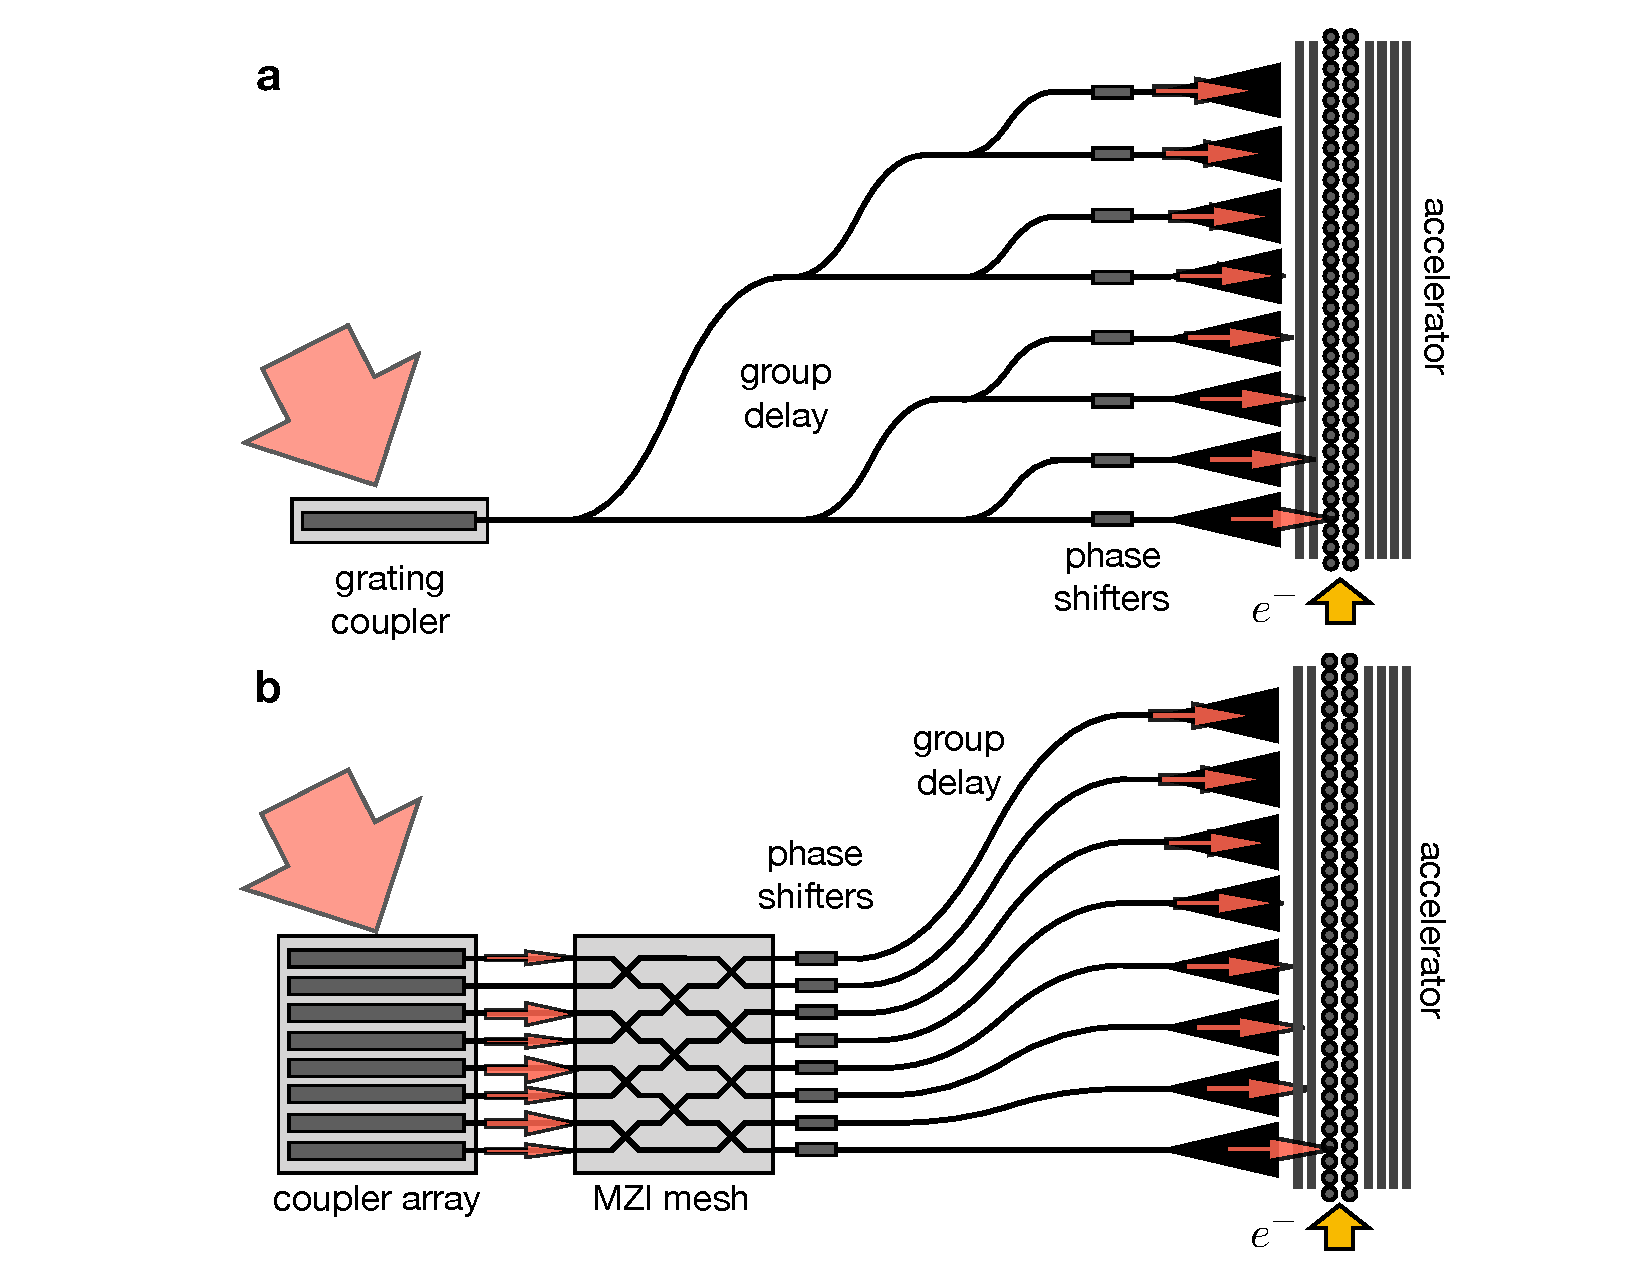
\includegraphics[width=\columnwidth]{figures/MZI_direct}
\caption{\label{fig:setup} \textbf{Schematic of the proposed DLA laser delivery control system.}  Comparison of setup from Ref \cite{hughes_-chip_2018} (\textbf{a}) and this work (\textbf{b}).  \textbf{a}, In the splitting structure of Ref. \cite{hughes_-chip_2018}, an input pulse (large red arrow) is focused to a single grating coupler on the chip surface.  The pulse is split a series of times and bends in the waveguide to create group velocity delay.  The phase of the pulses are corrected before injection into the accelerator.  \textbf{b}, In the schematic proposed in this work, the pulse is directly coupled into several waveguides through a grating coupler array. To mitigate the large variance in coupled powers, the pulses next enter a mesh of MZIs, which is sequentially adjusted, using the protocol from this paper, to provide uniform powers in each waveguide.  As before, phase control and group delay are performed using integrated phase shifters and lithographically-defined bends before couping to the accelerator channel.  The second scheme eliminates the damage and nonlinearity bottleneck present in $\textbf{a}$ directly after the input coupler.}
\end{figure}

Here we will give an overview of the proposed reconfigurable laser coupling scheme for DLA.  A schematic of our system is shown in Fig. \ref{fig:setup}.  The system consists of sequential stages for input coupling, power distribution, phase control, group delay control, and electron acceleration. 

In our design, the driving laser pulse is first focused onto an input element that directly splits the optical power into several waveguides.  Compared with schemes where the laser is first coupled to a single waveguide, as in the previous section, this coupling strategy can greatly improve the power that can be safely supplied by the driving laser. This element could take the form of a grating coupler array or combined grating coupler and power splitter geometry \cite{spuesens_grating_2016}.  Adjoint-based optimization techniques \cite{sapra2019inverse} may be employed to design novel input coupling components with improved coupling efficiency, less variation between powers, or significantly more output waveguides.

\begin{figure}
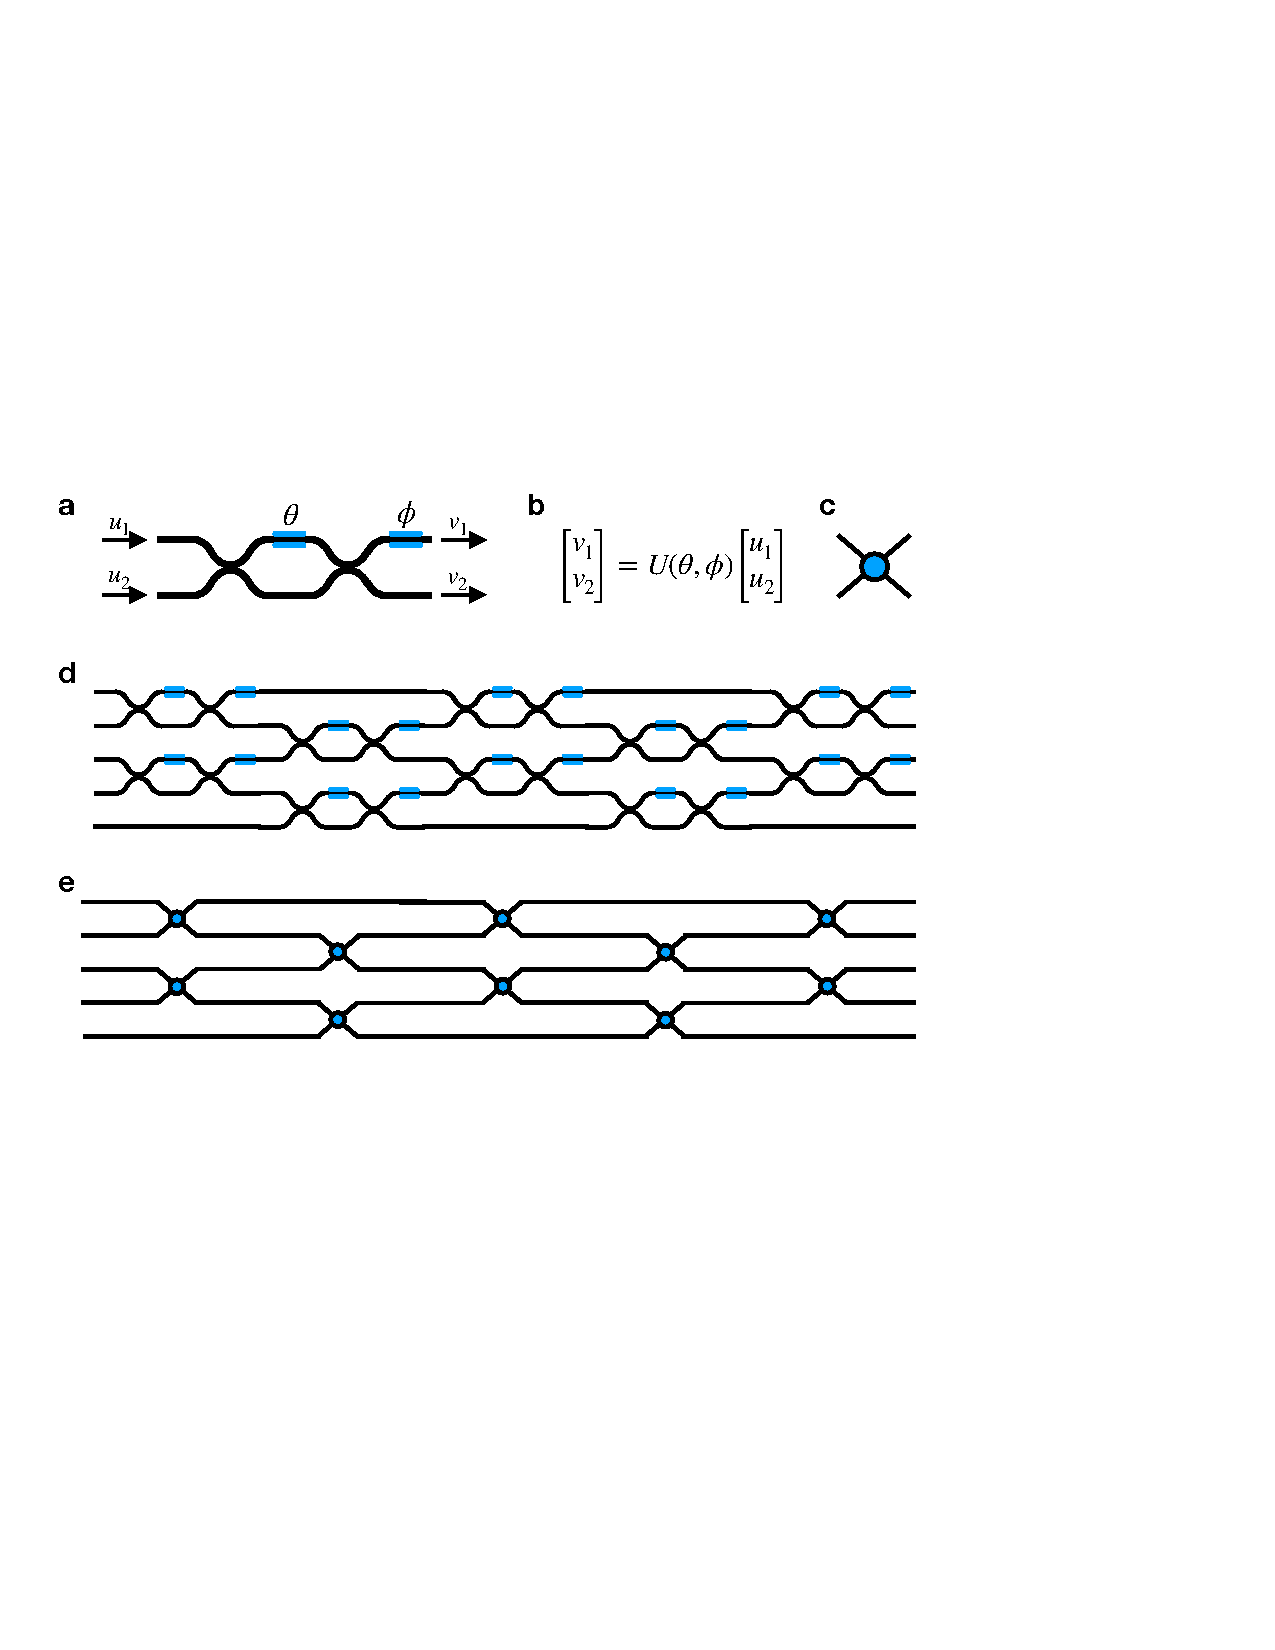
\includegraphics[width=1\columnwidth]{figures/MZI_MZI}
\caption{\label{fig:mesh} \textbf{Diagram of MZI mesh for power distribution.} \textbf{a}, Diagram of a single MZI consisting of two input ports and two output ports.  Where the two arms come together, a 50-50 beam-splitter operation is performed.  The blue regions indicate tunable optical phase shifters with added phases marked as $\theta$ and $\phi$.  \textbf{b}, The MZI represents a tunable unitary transformation on its inputs $[u_1, u_2]^T$ to give outputs $[v_1, v_2]^T$.  \textbf{c}, Simplified diagram representing an MZI in the following figures.  One may think of this element as a tunable power switch. \textbf{d}, Individual MZIs are combined into meshes, which may implement tunable unitary operations on several inputs.  Shown is a 'Clements' Mesh geometry, which was used in this work. \textbf{e}, Schematic of the Clements mesh in \textbf{d} using the simple MZI diagram in \textbf{c}.}
\end{figure}

After coupling, due to fabrication and alignment errors, there will be variation in the power distribution of each waveguide. To ensure that an equal amount of power is supplied to the accelerator, we introduce a power distribution component that is comprised of a mesh of MZIs.  As diagrammed in Fig. \ref{fig:mesh} \textbf{a}-\textbf{c}, each individual MZI is comprised of two beam-splitters and two optical phase shifters, $\theta$ and $\phi$, which can be electrically adjusted to perform the following unitary operation on its two inputs \cite{reck_experimental_1994,clements_optimal_2016,shen_deep_2017,pai2018matrix}
\begin{align}
\begin{split}
    \begin{bmatrix}
      v_1 \\ v_2
    \end{bmatrix}
    =&~U(\theta, \phi) 
    \begin{bmatrix}
      u_1 \\ u_2
    \end{bmatrix}
    \\
    =&~e^{i\frac{\theta}{2}} e^{i\frac{\phi}{2}}
    \begin{bmatrix}
      e^{i\frac{\phi}{2}}\cos{\frac{\theta}{2}} &
      e^{i\frac{\phi}{2}}\sin{\frac{\theta}{2}} \\
      - e^{i\frac{\phi}{2}}\sin{\frac{\theta}{2}} & 
      e^{-i\frac{\phi}{2}}\cos{\frac{\theta}{2}}
    \end{bmatrix}
    \begin{bmatrix}
      u_1 \\ u_2
    \end{bmatrix}.
\end{split}
\label{eq:U}
\end{align}
%

As shown in Figs. \ref{fig:mesh} \textbf{d},\textbf{e}, several MZIs may be combined in a mesh, which is capable of performing unitary operations over an arbitrary large number of inputs.  There are several possible configurations of the MZI mesh, each with their own benefits and drawbacks.  In this application, the mesh must be compact enough to fit on the chip and also have a bandwidth large enough to handle sub-picosecond pulses.  Whereas many meshes are capable of performing arbitrary unitary operations, for this power delivery problem it is only necessary to sort a single random input into a uniform output.  With these considerations in mind, the `Clements' mesh geometry \cite{clements_optimal_2016}, in which MZIs are configured in a rectangular mesh, is best suited for this application.   As diagrammed in Fig. \ref{fig:mesh} \textbf{d},\textbf{e}, the Clements mesh requires fewer layers than other designs \cite{reck_experimental_1994} and also is more robust to optical losses because of its symmetric layout.  Furthermore, it may be implemented in a `shallow' mesh with fewer layers than input ports.  This is especially useful for DLA power distribution problem as we will show that only a few layers are required for adequate power equalization.  %more details in supplementary?

The MZI meshes used in previous demonstrations \cite{annoni_unscrambling_2017, shen_deep_2017} were fabricated using Silicon waveguide platforms.  In these works, electrically controlled thermal heating was used to implement the tunable phase shifters.  In the system presented in this work, the presence of ultra-fast, high power pulses will introduce constraints on the fabrication.  For example, Si$_3$N$_4$ or SiO$_2$ materials would be preferred to Si for their high damage and nonlinearity thresholds.  Also, thermal phase shifters might suffer from drift or shot-to-shot variations when high power pulses are used.  While phase shifters using the electro-optic effect are another option, there may be unwanted interaction between the pulses and the phase shifter.  While these issues will explored in a future study, one promising option may be mechanical phase shifters \cite{han2015large} based on MEMS actuation, which are likely to be less sensitive to pulse propagation, more compact, and have a large enough bandwidth for DLA applications.

We will soon describe a sequential protocol for optimizing the Clements mesh for power distribution. As our protocol uses local information about the power within the network, we require the inclusion of integrated optical photodetectors within the MZI mesh, such as those used in \cite{annoni_unscrambling_2017}.  Alternatively, an imaging system, in conjunction with scattering elements, may be used to gather information about the power distribution from above the chip.

Once the power in each waveguide is equalized, we may use integrated optical phase shifters to correct the phase of each laser pulse such that it is synchronous with the electron beam. While the phase shifters may be adjusted to maximize energy gain, they may also be used to incorporate other functionality, such as beam focusing, total beam transmission, deflection, or diagnostics \cite{soong2014electron, ye2018deep}.  Beam energy measurements, performed periodically along the accelerator, may be used as a signal to automatically configure the optical phase shifters.

% \subsection{group delay}
Once the power and phase are sufficiently controlled, we must delay the laser pulse in each waveguide so that it arrives at the accelerator gap the same time as the moving electron beam. To do this, we introduce lithographically-defined bends in the waveguides to provide a delay that is matched to the electron arrival, producing the integrated optics analogue of a pulse-front tilt \cite{cesar_optical_2018}. The mathematical details of the bend design are described in the previous section.

% \subsection{DLA coupling}
The final stage involves coupling the waveguide mode into the acceleration channel.  Ideally, an inverse taper may be placed at the end of each waveguide to spread the mode area to match the spot size of the laser pulse to the dimensions of the DLA.  Then, an accelerator structure may be placed adjacent to the end of the waveguides.  Alternatively, the accelerator structures and tapers may be part of the same system and may be designed following ideas from proposed buried grating structures \cite{chang_silicon_2014}, or using inverse design techniques, such as what was shown Ref. \cite{hughes_method_2017} for free-space coupling.  Dielectric mirrors may be used to design the resonance of the acceleration cavity and provide back reflection if a single-sided drive is used \cite{yousefi2019dielectric} (as pictured in Fig. \ref{fig:setup}).  Ref. \cite{hughes_-chip_2018} argued that a moderately resonant acceleration cavity with quality factor of several hundred would be necessary to lower the input power to mitigate the input facet bottleneck introduced by that design.  However, in this proposal, because that bottleneck is eliminated, one might not require such a resonant structure.

\subsection{\label{sec:algo}Power Distribution Protocol}

With the control system defined, here we describe a power distribution protocol that may be implemented on a Clements mesh to optimally equalize the power coming from a random input source.  The goal of this power equalization stage is to find the settings of each of the integrated phase shifters such that, given an input to the mesh, there is an equal power in each output port.  A rudimentary implementation of this may involve performing a global optimization over each of the phase shifters.  However, when the number of degrees of freedom increases (for example, for a very large accelerator), this becomes unfeasible as the dimension of the search space scales linearly with the number of MZIs. Fortunately, the protocol presented in this work allows each MZI to be tuned individually and in sequence, layer by layer, from input to output.

\begin{figure}[htp]
\centering
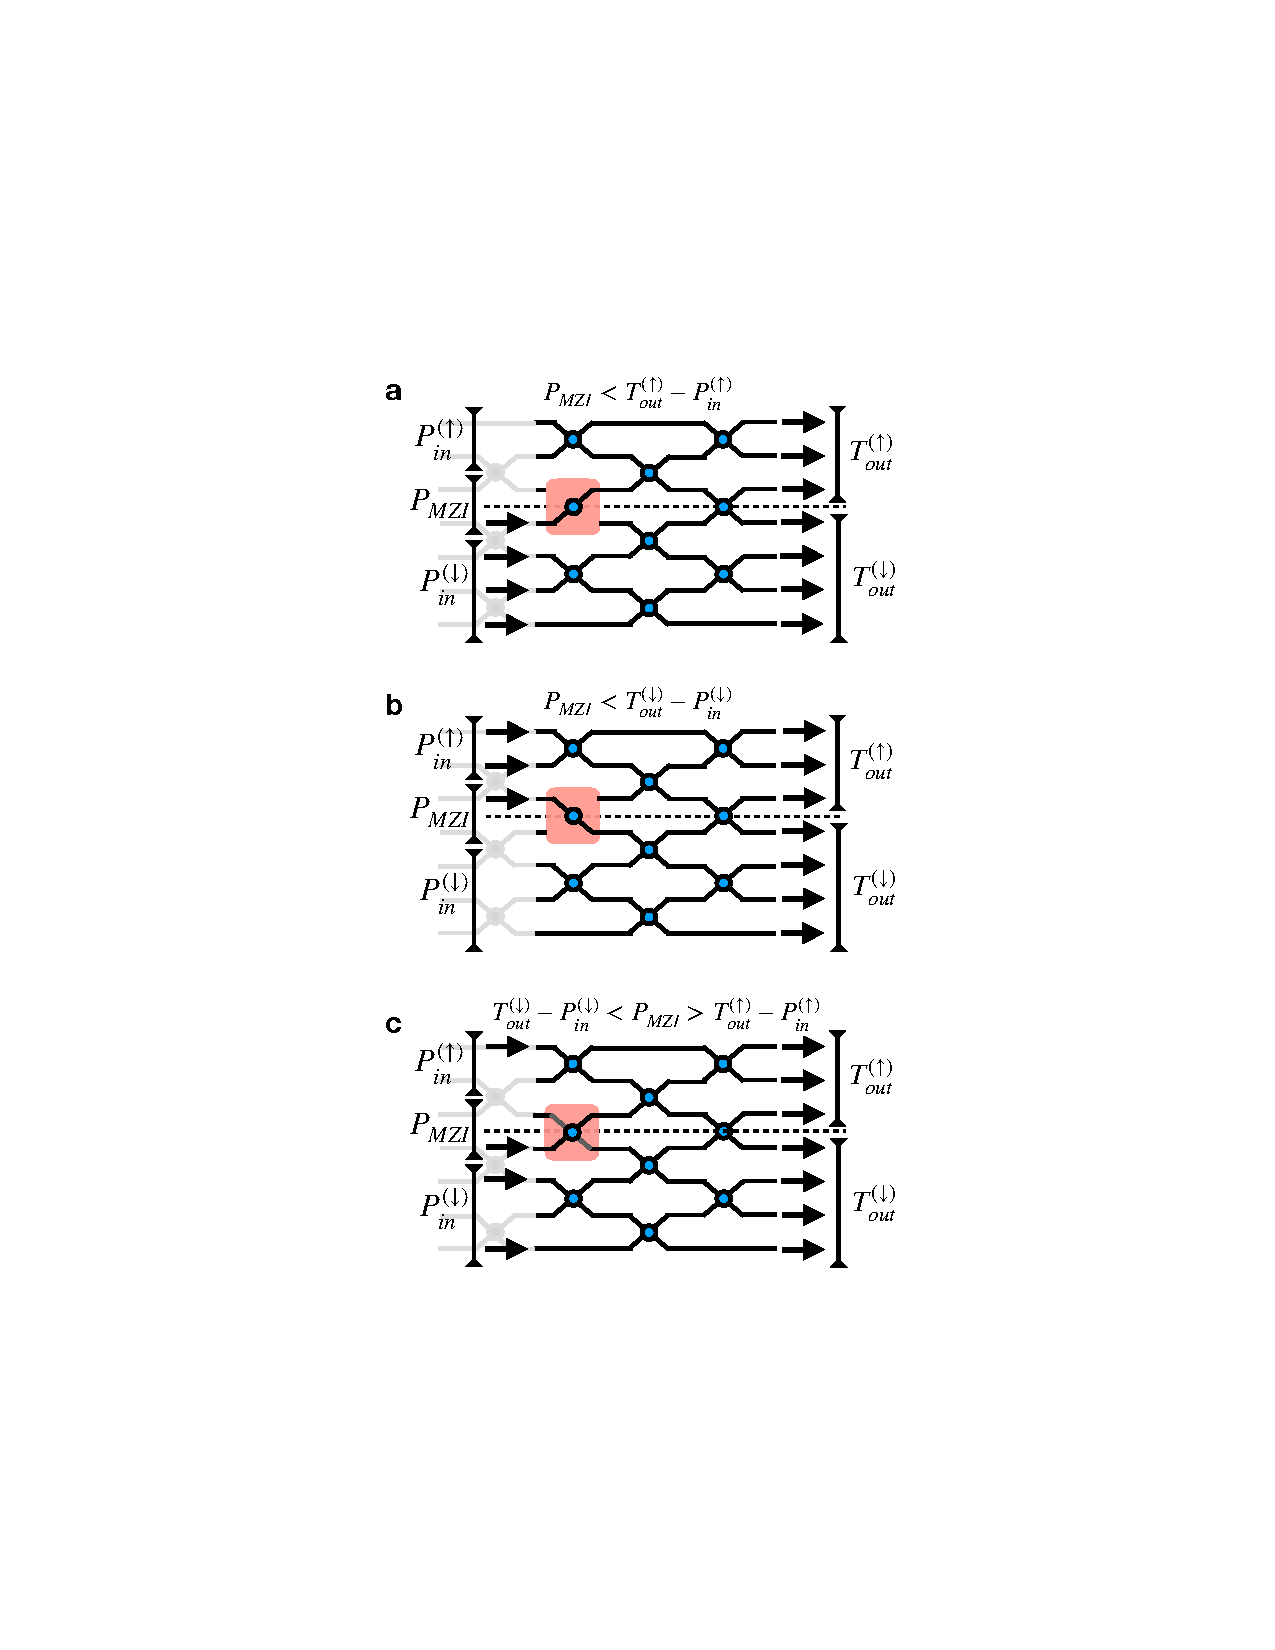
\includegraphics[width=0.6\columnwidth]{figures/MZI_tune}
\caption{\label{fig:algo} \textbf{Sequential algorithm for tuning single MZI.} The red square outlines the MZI being tuned.  Black arrows on the left indicate input power to the current layer, black arrows on the right indicate desired output powers (uniform in this case).  The dotted line separates the mesh into powers above and below the MZI.  \textbf{a} When there is more power needed in the ports above the MZI than are supplied in the ports leading into the MZI and above, the MZI should output all of its power to its top output port. \textbf{b} When there is more power needed in the ports below the MZI than are supplied in the ports leading into the MZI and below, the MZI should send all of its power to the bottom output port.  \textbf{c} In the intermediate case, the MZI should output just enough power to its top and bottom output ports to match the target power requirements.}
\end{figure}

Our protocol is diagrammed in Fig. \ref{fig:algo}, in which we show how to tune a single MZI (red) in a given layer of the network based purely on information about the powers coming into that layer.  For generality, we assume that we wish to tune this mesh to achieve an arbitrary target output power distribution $T_\textrm{out}^{(i)}$ for each of the $N$ ports $i~\in~\{1~..~N\}$.  Here in Fig. 3 the top port is at index $1$ and the bottom port is at index $N$.  We also assume that we have knowledge of the power at each of the ports coming into this layer, labelled $P_\textrm{in}^{(i)}$.

The essential idea of the protocol is to tune each MZI to locally direct power to either its top output port or its bottom output port depending on where power is deficient in the input to this layer and where it is needed in the final output layer. To visually represent this idea, in Fig. \ref{fig:algo}, we show a horizontal line bisecting the mesh through the MZI in question.  Assuming that the MZI is located vertically within the mesh with its top input  port at index $j$, we may define the sum of power input to this specific MZI as
%
\begin{equation}
    P_\textrm{MZI} \equiv P_\textrm{in}^{(j)} + P_\textrm{in}^{(j+1)}.
\end{equation}
%
The sum of the powers input to this layer both above and below this MZI, respectively, are defined as
%
\begin{align}
    P_\textrm{in}^{(\uparrow)} &\equiv \sum_{i=1}^{j-1} P_\textrm{in}^{(i)}\\
    P_\textrm{in}^{(\downarrow)} &\equiv \sum_{i=j+2}^N P_\textrm{in}^{(i)}.
\end{align}
%
Finally, the target powers above and below this MZI, respectively, are defined as
%
\begin{align}
    T_\textrm{out}^{(\uparrow)} &\equiv \sum_{i=1}^j T_\textrm{out}^{(i)} \\
    T_\textrm{out}^{(\downarrow)} &\equiv \sum_{i=j+1}^N T_\textrm{out}^{(i)}.
\end{align}
%
Now, using these values, we give a prescription for directing the power out of the MZI to optimally match the target.  We notice that there are three distinct cases to consider.  These are each diagrammed separately in the subplots of Fig. \ref{fig:algo}.  

Case 1 (Fig. \ref{fig:algo}\textbf{a}):  the sum of power supplied to the MZI and the ports \textit{above} it is less than the sum of power needed at the final output \textit{above} the MZI.  This is also written as
\begin{equation}
    P_\textrm{MZI} < T_\textrm{out}^{(\uparrow)} -  P_\textrm{in}^{(\uparrow)}.
\end{equation}
In this case, we require that the MZI direct all of its power to the \textit{top} output port, as shown in the red box of Fig. \ref{fig:algo}\textbf{a}.

Case 2 (Fig. \ref{fig:algo}\textbf{b}):  the sum of power supplied to the MZI and the ports \textit{below} it is less than the sum of power needed at the final output \textit{below} the MZI.  This is also written as
\begin{equation}
    P_\textrm{MZI} < T_\textrm{out}^{(\downarrow)} - P_\textrm{in}^{(\downarrow)}.
\end{equation}
In this case, we require that the MZI directs all of its power to the \textit{bottom} output port, as shown in the red box of Fig. \ref{fig:algo} \textbf{b}.

Case 3 (Fig. \ref{fig:algo}\textbf{c}):  when neither of the two cases above are satisfied, i.e.:
\begin{align}
\begin{split}
    P_\textrm{MZI} &\geq T_\textrm{out}^{(\uparrow)} -  P_\textrm{in}^{(\uparrow)} ~~~~~\textrm{and} \\
    P_\textrm{MZI} &\geq T_\textrm{out}^{(\downarrow)} - P_\textrm{in}^{(\downarrow)},
\end{split}
\end{align}
we require the MZI only supply $T_\textrm{out}^{(\uparrow)} - P_\textrm{in}^{(\uparrow)}$ of its power to the top port.  The leftover power may be transmitted to the down port, which, by power conservation, will be equal to $T_\textrm{out}^{(\downarrow)} - P_\textrm{in}^{(\downarrow)}$ since $\sum_{i=1}^{N}P_\textrm{in}^{(i)} = \sum_{i=1}^{N}T_\textrm{out}^{(i)}$.  This is demonstrated in Fig \ref{fig:algo}\textbf{c} where the MZI performs a partial splitting of power.

With this protocol, one may thus optimize each MZI sequentially through the mesh.  To do this optimally, the MZIs must be tuned layer-by-layer from input to output.  Within each layer, a set of integrated photodetectors must be used to measure $P_\textrm{in}^{(i)}$ for all ports $i$.  Then, the individual MZIs in this layer may be tuned in parallel or in any order desired.

While the algorithm presented above assumes lossless components, in practice, variations in loss between MZIs in each layer will introduce discrepancies between the expected and measured output power.  Therefore, to compensate for this, in practice, a calibration of each MZI’s loss, and corresponding update to the algorithm, may be necessary to achieve good performance.

\subsection{\label{sec:demo}Numerical Demonstration}

\begin{figure}[htp]
\centering
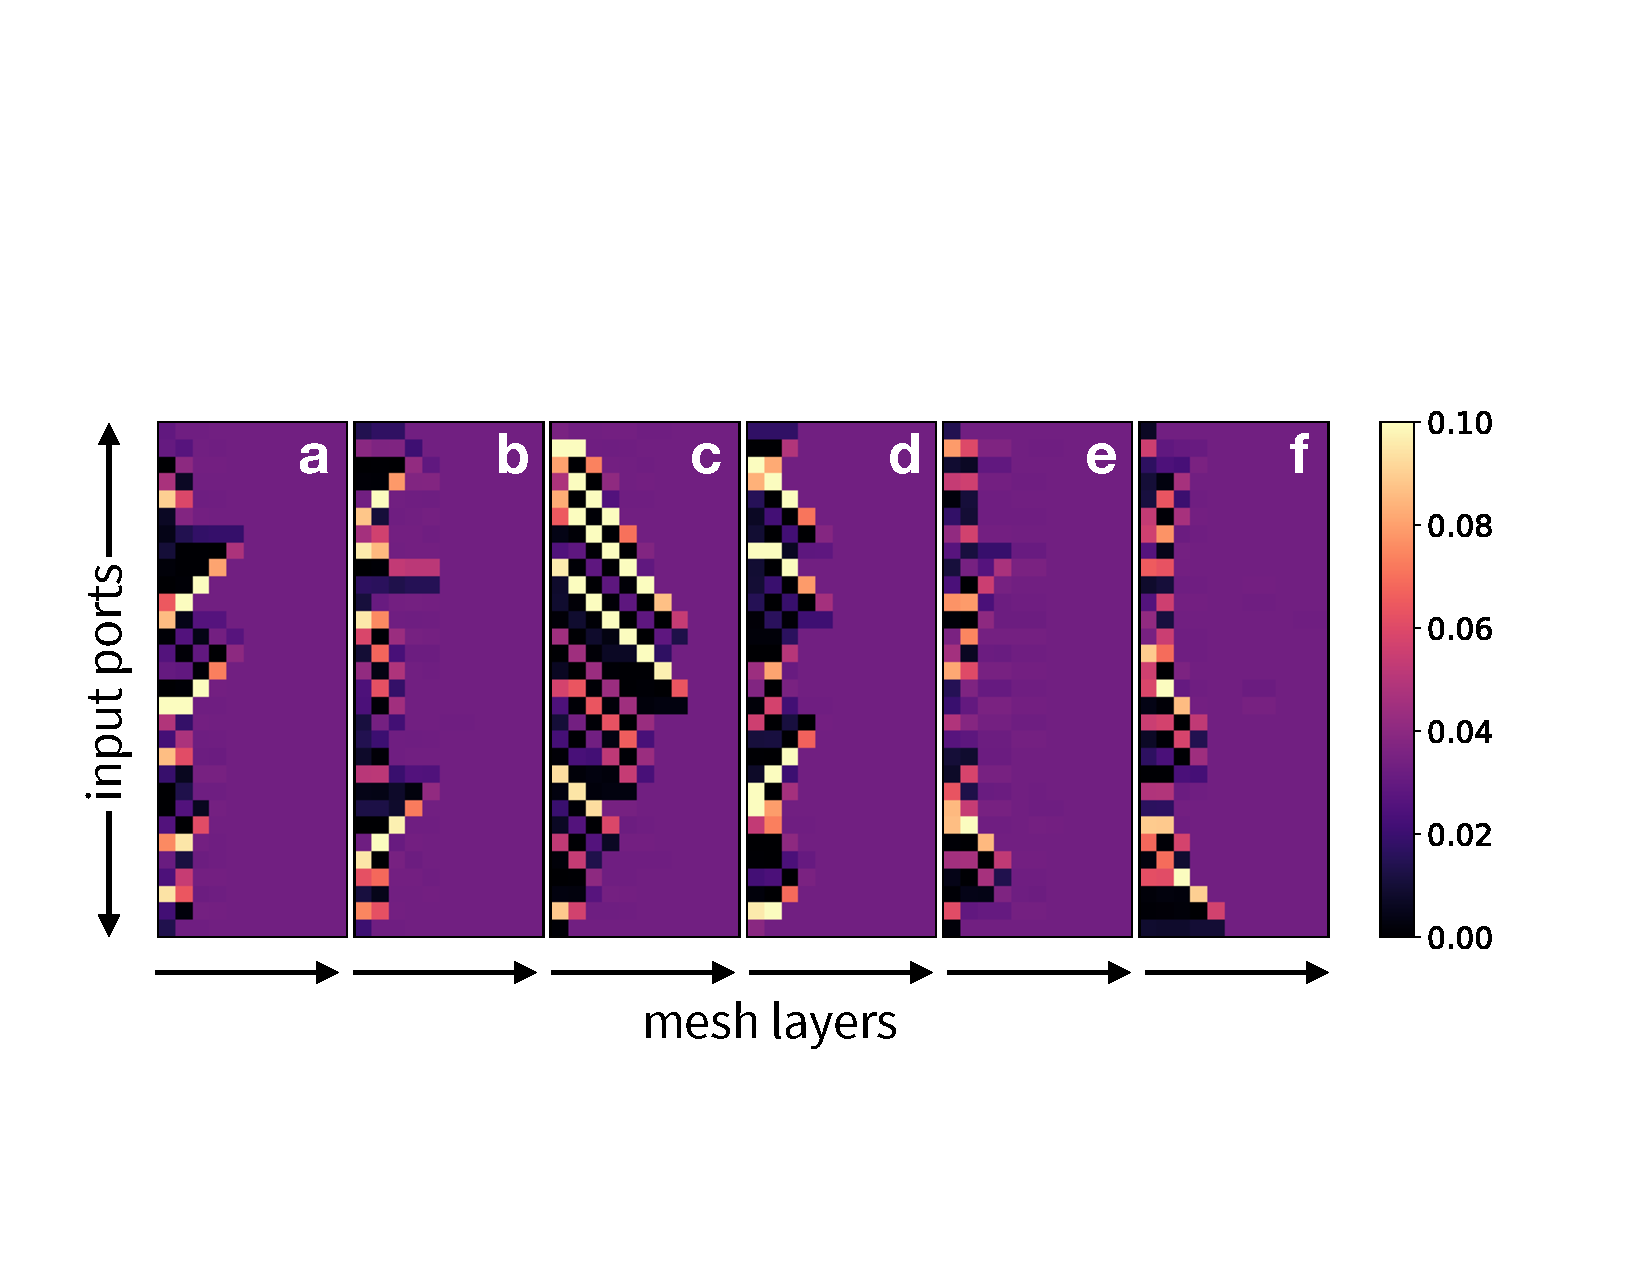
\includegraphics[width=1\columnwidth]{figures/MZI_random}
\caption{\label{fig:equalization} \textbf{Demonstration of mesh optimization for equal power distribution.} \textbf{a}-\textbf{f} The powers in each port after optimizing the mesh for uniform output power given several random input powers.  The colorbar represents the fractional power in each port, where the total power is normalized to 1. The vertical axis represents the input port index and the horizontal axis represents the layer index.  Power flows from left to right.  Equalization is achieved, on average, after only around 5 layers given this network with 30 ports.}
\end{figure}

To demonstrate our protocol, we perform numerical simulations of a Clements mesh and optimize it for power equalization from random inputs to uniform outputs. A software package \cite{hughes2018DLA_Control} was written to simulate the mesh and perform the optimizations. This package was written such that it may eventually be augmented to interface with a physical MZI mesh to act as a control mechanism.  The result of 6 independent runs is shown in Fig \ref{fig:equalization}, in which we plot the power in each port within the network after it is optimized using this procedure.

For each run, we initialize a Clements mesh with $N = 30$ input ports and $M = 10$ layers.  Then, we generate a vector of random input powers to couple to the mesh, $P_\textrm{in}$.  When constructing $P_\textrm{in}$, each element is chosen uniformly at random between 0 and 1 and then the whole vector is normalized such that it sums to 1.  The phase of each input mode is set to 0.  For demonstration purposes, we optimize the mesh to output to a uniform output target $T_\textrm{out}$, where each element of $T_\textrm{out}$ is equal to $1/N$, such that both the input and target powers are normalized to each sum to 1.  Although a uniform output target was chosen as it is most applicable to DLA applications, the same protocol may be equally applied to other targets with similar results.

We then step through the mesh from input to output, tuning all MZIs in a given layer according to the protocol introduced in the previous section before moving to the next layer.  To perform the tuning, we use a simple downhill simplex algorithm \cite{avriel_nonlinear_2003} to tune the phase shifters ($\theta$ and $\phi$ in Eq. \ref{eq:U}) in the MZI until they output the correct power as described by the protocol.  From Fig. \ref{fig:equalization}, we notice that equalization is achieved after only around 5 layers on average.

To understand how the device operation scales with the number of layers, we studied the performance of the equalization routine as the number of ports are increased.  The results are shown in Fig. \ref{fig:scaling} where we show the mean-squared-error between the power in each layer, defined as 
\begin{equation}
    MSE = \frac{1}{N}\sum_{i=1}^N \left( P_\textrm{in}^{(i)} - T_\textrm{out}^{(i)} \right)^2.
\end{equation}
We then sweep through different mesh sizes and average the data for each mesh over 5 runs with different random inputs.  The number of layers needed for equalization grows slowly as the network size is increased.  This suggests that for very large networks (with $>$ 100-1000 ports), only tens of layers of MZIs may be needed in the Clements mesh to perform power equalization.

As evidenced by Fig. \ref{fig:equalization}, extreme input conditions, such as the full power concentrated at a single port on the edge of the mesh, will need a full quadratic mesh to fully equalize power.  However, these edge cases are not only far less likely than the more uniform input conditions, but also represent failure modes caused by severely distorted input laser modes, which are likely to damage the structure.  In practice, we therefore do not expect the MZI mesh to compensate for them.

\begin{figure}
\centering
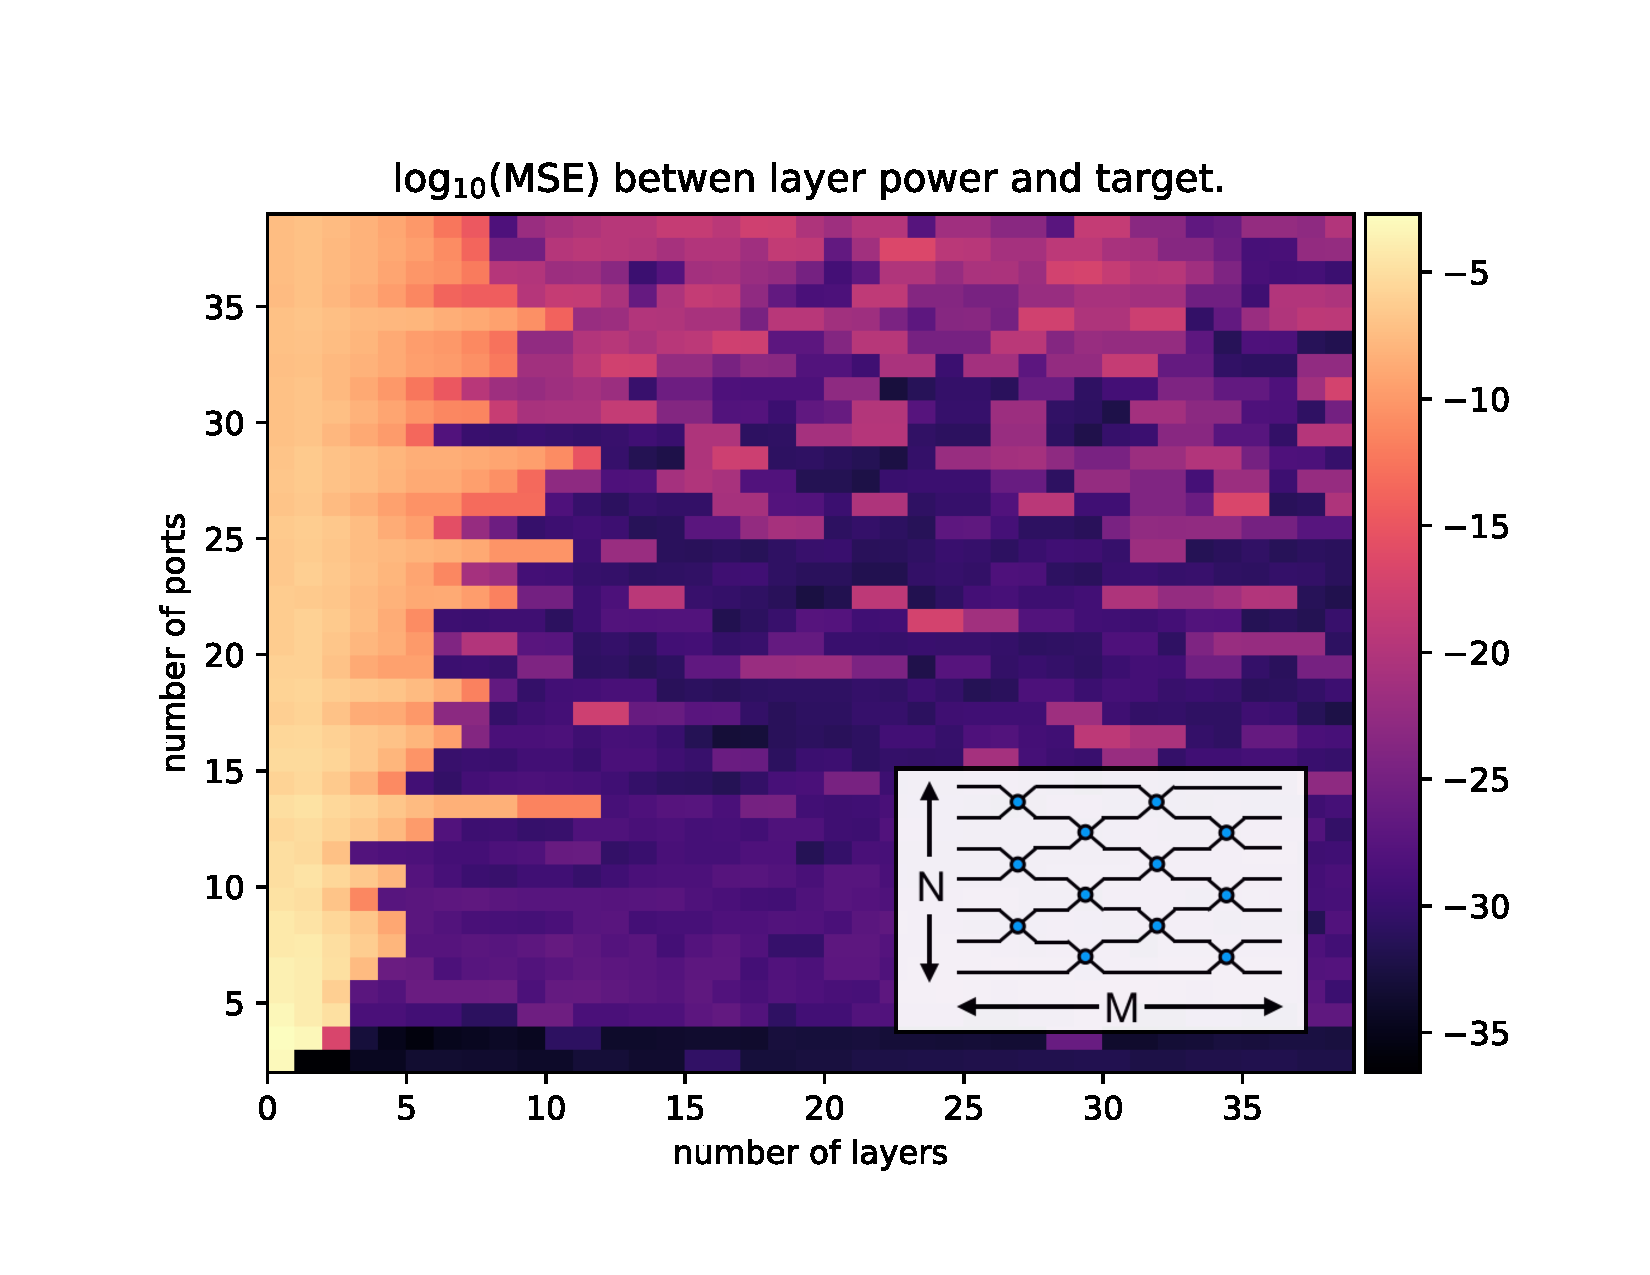
\includegraphics[width=1\columnwidth]{figures/MZI_scale}
\caption{\label{fig:scaling} \textbf{Analysis of mesh performance vs. number of input ports}.  We plot the mean-squared-error between the power in each layer and the target power after the mesh has been optimized.  These are averaged over 5 random input values.  We see that the number of layers ($M$) needed to equalize the power in the mesh increases slowly with respect to the number of ports ($N$).}
\end{figure}

\subsection{\label{sec:DLA_analysis}Performance Improvement}

To quantify the benefit of this new power distribution component, we now compare the performance of a DLA with the power splitting approach of Ref. \cite{hughes_-chip_2018} to one with direct coupling and power control from this work and as diagrammed in Fig. \ref{fig:setup}.  For each of these approaches, we give an estimate of the acceleration gradient, number of output waveguides, and acceleration length needed to achieve a given energy gain with a single driving laser.  

Following the analysis of Ref. \cite{hughes_-chip_2018}, we first consider a splitting design in which a single input waveguide is split $N_s$ times to cover the full length of acceleration.  We assume that an optical pulse with energy $\Ud$ and temporal duration $\tau$ is coupled into the input waveguide.  We must ensure that $\Ud$ is below the damage and nonlinearity limit of the waveguides, which was recently measured to be 20 nJ in SiN waveguies using pulses of duration of 250 fs \cite{tan2019silicon}.  This corresponds to a fluence of 0.12 $J/cm^2$ for a mode area of 17.2 $\mu m^2$, as used in this reference. We then assume that this initial waveguide is split $N_s$ times, in a binary fashion, to couple to $N = 2^{N_s}$ final waveguides, which are directly coupled to the accelerator. The power coupling efficiency factors corresponding to waveguide splitting and bending loss are denoted by $\eta_s$ and $\eta_b$ respectively. The values used for these efficiencies are given in Table \ref{tab:params} and are consistent with those of Ref. \cite{hughes_-chip_2018}.

Next, we assume each waveguide powers $\Np$ periods of the accelerator, each of height $h$ and width $\beta \lamo$ to satisfy the synchronicity condition, where $\beta$ is the ratio of the electron speed to the speed of light and $\lamo$ is the free space wavelength of the driving laser.  This gives a total acceleration length of
%
\begin{equation}
    L = N \Np \beta \lamo
    \label{eq:L}
\end{equation}

In terms of these parameters and  the peak electric field of the laser pulse incident on the accelerator channel $(E_0)$, the corresponding power intercepting the DLA is $P_0 \simeq \zeta E_0^2 h N_p \lambda \beta n/ (2 Z_0)$, where $Z_0 = 377 \Omega$ is the impedance of free space, $n$ is the refractive index, and $\zeta$ is a dimensionless factor of order unity (for a Gaussian $\zeta = \pi/2$). Considering losses between the input coupling of a pulse with energy $U_d$ and duration $\tau$, we may compute an expression for $P_0$ and solve for $E_0$ to obtain
\begin{equation}
    \Eo = \sqrt{\frac{2 \Ud Z_0 (\eta_s \eta_b)^{N_s}}{2^{N_s} \zeta \Np \tau \lamo \beta h n}},
    \label{eq:E0}
\end{equation}

The acceleration gradient, defined as the energy gain ($\DE$) per unit length, may be written in terms of the acceleration length $L$, input electric field $\Eo$, and elementary charge $e$ as

\begin{equation}
    G = \frac{\DE}{eL} = \kappa \Eo,
    \label{eq:G}
\end{equation}
%
The proportionality constant or \textit{structure factor} $\kappa$ is a dimensionless quantity that denotes the coupling of incident field to the structure. Structure factors of $\kappa = 0.2$ have been experimentally demonstrated \cite{cesar_optical_2018} and $\kappa = 1.34$ theoretically predicted \cite{bar2019design} for various structure designs, and by use of a resonant structure with a quality factor $Q$ it can be further enhanced as $\sqrt{Q}$ \cite{hughes_-chip_2018}. We here assume a moderate value of $\kappa = 1$. With the expression above for the gradient, along with Eqs. (\ref{eq:L}) and (\ref{eq:E0}), we may solve for the number of waveguide splits required to accomplish the energy gain of $\DE$ as
\begin{equation}
    N_s = \log_2 \left[ \frac{\DE^2 \tau h n \zeta}{2  \kappa^2 \Ud \Np \beta \lamo Z_0} \right] / \log_2 (2 \eta_s \eta_b)
    \label{eq:N}
\end{equation}
The total number of waveguides feeding the DLA is then $N = 2^{N_s}$. We can see that in the limit where the efficiency terms are equal to unity, $N$ reduces to the quantity contained inside the first logarithm in Eq. (\ref{eq:N}).

In contrast, using a direct coupling method with power distribution components introduced in this work, there is no need for on-chip splitting of the optical power.  Because of this, we may couple $\eta_\textrm{MZI} \times \Ud$ of optical energy separately into each waveguide, where $\eta_\textrm{MZI}$ is the throughput efficiency of the MZI. In the experimental demonstrations of Ref. \cite{annoni_unscrambling_2017,shen_deep_2017}, less than 50\% of power loss was demonstrated for a 4-layer MZI mesh. As a conservative estimate, we assume here $\eta_\textrm{MZI} = 0.25$ for 10 layers.  Additionally, negligible amounts of reflection and internal backscattering were observed in these implementations, and therefore are not considered in this analysis.  Following a similar analysis, the electric field incident on the accelerator, given by Eq. (\ref{eq:E0}), loses its $N$ dependence and thus the number of required output waveguides needed scales as 
\begin{equation}
    N^{(\textrm{direct})} =  \frac{\DE}{\kappa} \sqrt{\frac{\zeta \tau h n}{2 \Ud \eta_\textrm{MZI} \Np \beta \lamo Z_0 }}.
    \label{eq:N_direct}
\end{equation}

In Fig. \ref{fig:plots} we show the scaling of the acceleration gradient, number of output waveguides, and acceleration length as a function of required energy gain for a DLA given realistic parameters, which are supplied in Table \ref{tab:params}.  Based on previous demonstrations of these components \cite{annoni_unscrambling_2017, shen_deep_2017} the reflection and backscattering is negligible, and therefore not considered in this analysis.

To connect these results with prior work, we note that for the split waveguide approach, Eqs. (\ref{eq:L}), (\ref{eq:E0}), (\ref{eq:G}), (\ref{eq:N}) give nearly identical results as those of the more involved analysis of \cite{hughes_-chip_2018} for the case of silicon nitride waveguides for a single-stage energy gain of 20 keV, when the same input parameters are used. 
In Ref. \cite{tan2019silicon}, the damage and nonlinearity constraints using similar pulse parameters was studied experimentally. It was found that a silicon nitride waveguide could sustain a pulse of 20 nJ for several milimeters of propagation distance.  Therefore, while this proposed power equalization system includes more components (beam splitters and phase shifters), it is likely to be well within the damage threshold.

However, the results in Fig. \ref{fig:plots} for the split waveguide approach (solid blue curves) are somewhat more optimistic than those of the prior work, as recent experiments \cite{tan2019silicon, bar2019design} have provided evidence for larger values of $U_d$ and $\kappa$ than were previously assumed. These more optimistic parameters are reflected in Table \ref{tab:params_MZI}. However, due to the $N_s$ scaling of the power loss for the split waveguide approach, higher energy gains per stage rapidly become prohibitive as the resulting gradient drops exponentially and the number of required waveguides increases. In Ref. \cite {hughes_-chip_2018} this difficulty was addressed by cascading multiple laser-coupled stages in series to achieve a reasonable energy gain of 1 MeV.  In contrast, as seen in Fig. \ref{fig:plots} the direct coupling approach can in principle achieve this with one acceleration stage and one input laser, requiring 144 waveguides over a length of 2.8 mm with a gradient of 350 MeV/m. These are promising numbers for a DLA structure and may be improved primarily by optimizing for higher values of $\kappa$ and $\Np$, which may be accomplished using inverse design techniques \cite{hughes_method_2017}.

\begin{table}[!h]
% Table captions go at the top.
\centering
\begin{tabular}{lccc}
\hline
Metric & Description & Value & Units \\
\hline
$\beta$ & $e^{-}$ speed / $c_0$ & 1 & - \\
$\lamo$ & free space wavelength & 2 & $\mu$m \\
$\Np$ & \# DLA periods / waveguide & 10 & - \\
$\kappa$ & structure coupling factor & 1 & - \\
$\Ud$ & input pulse energy & 20 & nJ \\
$\tau$ & input pulse duration & 250 & fs \\
$h$ & DLA structure height & 2 & $\mu$m \\
$n$ & waveguide refractive index & 2 & - \\
$\eta_s$ & waveguide splitting efficiency & 0.95 & - \\
$\eta_b$ & bend loss efficiency & 0.95 & - \\
$\eta_\textrm{MZI}$ & MZI transmission efficiency & 0.25 & - \\
$\zeta$ & geometrical mode factor & $\pi$/2 & - \\
\hline
\end{tabular}
\caption{\label{tab:params_MZI} Set of parameters used in the analysis of Fig. \ref{fig:plots}}.
\end{table}

\begin{figure}[!h]
\centering
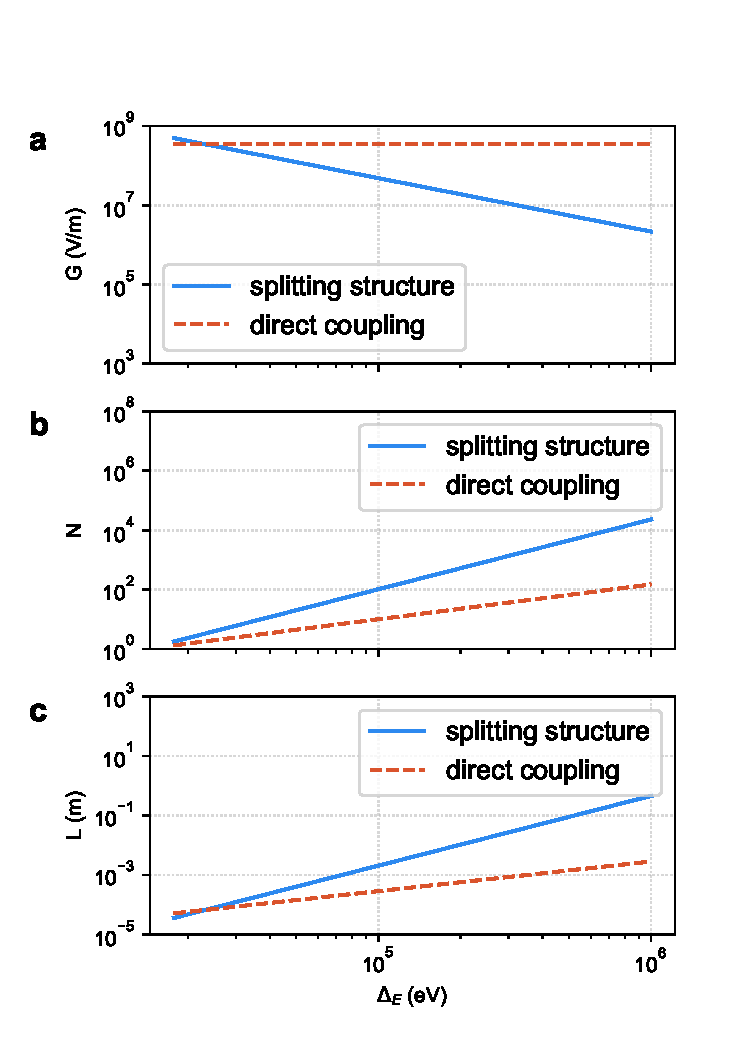
\includegraphics[width=0.7\columnwidth]{figures/MZI_param}
\caption{\label{fig:plots} \textbf{Figure of merit scaling for different laser coupling architectures.} Solid blue lines refer to the results using the system of Ref \cite{hughes_-chip_2018}, in which all optical power is initially coupled at a single input facet. Red dotted lines refer to the structure from this work.  \textbf{a}  The acceleration gradient as a function of electron energy gain.  For the splitting structure, the acceleration gradient diminishes rapidly as the length of acceleration is increased to match the desired energy gain.  However, the structure from this work achieves uniform gradient in principle.  \textbf{b}  The number of output waveguides ($N$) required to achieve an given energy gain of $\DE$.  \textbf{c}  The acceleration length ($L$) required to achieve an given energy gain of $\DE$.}
\end{figure}


Our proposal provides a method for automated control of DLA systems and eliminates the major issues with previous laser coupling schemes.  We show that MZI meshes are a promising candidate for a power distribution system for DLA and our findings may be applied to other applications in integrated optics requiring power routing.  The proposal given here only uses existing optical components and, therefore, should be feasible for an experimental demonstration.

The procedure we introduce for optimizing the MZI mesh to achieve arbitrary power distribution is highly efficient in terms of number of measurements and phase shifter tunings.  For a mesh with $N$ ports and $M$ layers, our protocol replaces one large optimization problem with $2NM$ degrees of freedom to $MN$ independent optimization problems with 2 degrees of freedom each.  This greatly improves the feasibility of implementing this protocol on large meshes with thousands of input ports, for example, which may be needed for large-scale DLA.  In comparison with other mode sorting schemes \cite{annoni_unscrambling_2017, miller_self-aligning_2013} in which a Reck (triangular) mesh architecture is used, our algorithm provides the opportunity to perform similar functionality on a rectangular mesh, which benefits from more uniform loss and bandwidth across pathways through the device.

We show that a shallow Clements mesh is sufficient for equalizing power from random inputs.  This is of crucial importance for DLA applications where there are limitations on the chip space available for phase shifters and electrical contacts.  It also means that a shorter propagation length within the waveguides can be achieved, which reduces the possible nonlinear effects.  Having a shallow mesh also allows the device to retain a large bandwidth, which decreases with the number of MZIs in an optical path.  This is crucially important for handling sub-picosecond driving pulses used in DLA.  However, the bandwidth of MZI meshes and its scaling with respect to network size is not yet fully understood.  This will need to be tested experimentally or with a separate numerical study.

The optimization protocol presented here decomposes the global optimization problem of tuning the entire mesh into several subproblems involving tuning the individual MZIs.  However, alternatively a gradient-based approach may potentially be used to train the full mesh.  It was shown previously \cite{hughes2018training} that the gradient of the output of an MZI mesh with respect to the dielectric function of each of the phase shifters may be measured experimentally using adjoint fields \cite{veronis_method_2004}. Interestingly, for the case of maximizing the acceleration of a DLA, it was independently shown that the corresponding adjoint fields are given exactly by the fields radiated by the electron beam \cite{hughes_method_2017}.  This suggests an interesting approach to optimizing the MZI mesh towards maximum acceleration by first measuring the radiation from test electron beam, and then using the protocol from Ref. \cite{hughes2018training} to measure the derivative of the acceleration with respect to each of the phase shifters.  With this, one may do parallel, gradient-based updates of the phase shifters and optimize arbitrarily large grids with high efficiency. This idea may be explored in a future study.

Overall, these studies indicate that integrated optical power delivery systems are worth continuing to pursue for DLA.  We presented a path towards automatic power distribution, which is an essential component towards scaling DLA to longer length scales and exciting applications.  We also provide a novel application of the MZI mesh, which is already finding many applications in other exciting reconfigurable optics applications.  Our efficient protocol for optimizing an MZI for arbitrary power distribution may also find many applications beyond DLA.

\section{\label{sec:discussion}Outlook and Conclusions}


Integrated optics, and reconfigurable optics in general, allows unique opportunities for accelerators on a chip to take advantage of high precision control and automatic compensation for errors from fabrication, alignment, or drift. These studies presented two promising avenues for accomplishing extended acceleration lengths for these accelerators and eventually may enable future applications of DLA technology.

Since publishing, recent works have further validated the feasibility and usefulness of using integrated optics platforms as a power delivery system for DLA. A recent study \cite{zhao_design_2018} proposed the use of dieletric waveguides as a co-propagating accelerating scheme.  Here, the optical pulses are coupled into a slot waveguide configuration and the evanescent fields are used to provide energy gain to the electron beams.  The waveguide widths are tapered along the propagation axis, which allows for phase matching to an accelerating, subrelativistic electron beam.  
Furthermore, experimental damage and nonlinearity testing of SiN waveguides has shown that the waveguides may sustain pulses similar to those used in these parameter studies \cite{tan2019silicon} without damage or significant nonlinear effects.
Finally, recent demonstrations of the first waveguide-coupled DLA were performed using a grating coupler and accelerator structure designed using inverse design \cite{sapra2019inverse,sapra_-chip_2019}.
Further experimental studies are underway, with the goal of realizing a multi-stage integrated accelerator within the next two years.


\chapter{Training of Optical Neural Networks}
%!TEX root = ../main.tex

\section{Introduction to Machine Learning}

\subsection{Applications}

\subsection{Hardware Demands}

\section{Linear Nanophotonic Processors}

\section{Optical Neural Networks}

\subsection{Conventional Neural Network}

\subsection{Optical Integration}

\subsection{Training Protocols}

\subsubsection{Computer Model Training}

\subsubsection{Brute Force Training}

\section{In Situ Backpropagation Training}

\subsection{Derivation Using Adjoint Method}

\subsection{Method for Measurement of Adjoint Gradient}

\subsection{Numerical Demonstrations}

\section{Electro-Optic Activation Functions}

\subsection{Motivation}

\subsection{Proposed Activation Function}

\subsection{Scaling Laws}

\subsection{Demonstration}

\section{Wave-Based Analog Recurrent Neural Networks}

\subsection{Wave Equation vs. Recurrent Neural Network}

\subsection{Vowel Classification through Wave Propagation}


\chapter{Extension of Adjoint Method beyond Linear Time-Invariant Systems.}
%!TEX root = ../main.tex

\section{Nonlinear Devices}

\subsection{Generalization of Adjoint Method to Nonlinear Problems}

\subsection{Inverse Design of Nonlinear Photonic Switches}

\section{Active Devices}

\subsection{Adjoint Sensitivity for Multi-Frequency FDFD Problems}

\subsection{Inverse Design of Optical Isolators through Dynamic Modulation}

\section{Adjoint for Time Domain}

\subsection{Derivation}

\subsection{Challenges}

\section{Forward-mode Differentiation}


\chapter{Conclusion and Final Remarks}
%!TEX root = ../main.tex



% ================ APPENDIX =================== %

\appendix
\chapter{Something}
Some appendix section.

% ============== BIBLIOGRAPHY ================= %

\bibliographystyle{plain}
\bibliography{bib/thesis_bib, bib/DLA_bib}

\end{document}